\documentclass[12pt]{article}

\usepackage[margin=50pt]{geometry}
\usepackage{amsmath}
\usepackage{graphicx}
\usepackage{systeme}
\usepackage{enumitem}

\graphicspath{/images}
\geometry{footskip=0.8cm}

\title{Operations Research Case Studies}
\author{Thomas Vroom}

\begin{document}
\maketitle

%
% Topic 1 - Coin Flipping
%
\section{Coin Flipping}
Suppose we have a fair coin with two sides, $H$ and $T$.
What is the expected number of coin flips until we see the first $H$?
Let $X$ be the number of flips until we see the first $H$:

\begin{table}[h]
    \centering
    \begin{tabular}{c|c|c|c|c|c|c}
    $x$ & 1 & 2 & 3 & 4 & ... & $k$ \\ \hline
    $P(X = x)$ & $\frac{1}{2}$ & $\frac{1}{4}$ & $\frac{1}{8}$ & $\frac{1}{16}$ &  & $\frac{1}{2^k}$
    \end{tabular}
\end{table}

\noindent
If we sum this series, we eventually get that the expected number of flips until the first $H$ is 2.
Note that 2 is also the inverse of the probability of getting $H$ on the first flip.

\noindent
\\
Let's take another example: 
What is the expected number of flips until we see $HT$?
We can create a similar table as before, but this will quickly become too complex.
Instead, we can model this problem as a \textbf{Markov Chain}:

\begin{figure}[h]
    \centering
    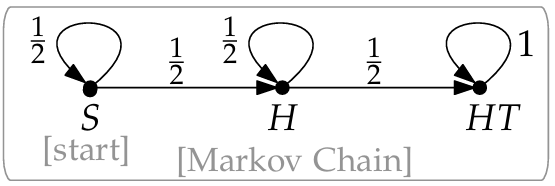
\includegraphics[scale=0.75]{images/markovchain1.PNG}
\end{figure}

\noindent
Let $E_x$ be the expected number of flips to go from state $x$ to state $HT$.
We can model this Markov chain as the following system of linear equations:
\begin{equation*}
    \begin{split}
        E_S & = 1 + \frac{1}{2}E_S + \frac{1}{2}E_H \\
        E_H & = 1 + \frac{1}{2}E_H + \frac{1}{2}E_{HT} \\
        E_{HT} & = 0
    \end{split}
\end{equation*}

\noindent
Note that the first 1 is there because you need to flip a coin to progress to the next state anyway.
When solving this system of equations, we find that $E_S = 4$.
This is once again the inverse of the probability of getting $HT$ straight away.

\newpage
\noindent
Next, let's consider the expected number of flips until we see $HH$.
We can model this using the following Markov chain:

\begin{figure}[h]
    \centering
    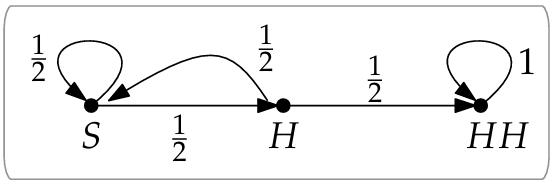
\includegraphics[scale=0.75]{images/markovchain2.PNG}
\end{figure}
\vspace{-0.75cm}
\begin{equation*}
    \begin{split}
        E_S & = 1 + \frac{1}{2}E_S + \frac{1}{2}E_H \\
        E_H & = 1 + \frac{1}{2}E_S + \frac{1}{2}E_{HH} \\
        E_{HH} & = 0
    \end{split}
\end{equation*}

\noindent
Solving this system of equations, we find that $E_S = 6$.
However, this is not the inverse of the probability of getting $HH$ straight away.

\subsection{First Passage / Recurrence Time}
The truth is that we actually measured two different things:

\begin{itemize}
    \item $E_x$ (i.e. the system of equations) measures the number of coin flips before we see a sequence for the first time.
    This is called \textbf{First Passage Time}.
    \item The inverse of the probability measures the number of coin flips before the process returns to the same state.
    This is called \textbf{Recurrence Time}.
\end{itemize}

\noindent
The reason that these two are different is because they measure completely different Markov chains:

\begin{figure}[h]
    \centering
    \begin{minipage}{.5\textwidth}
      \centering
      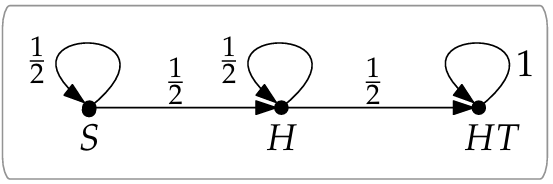
\includegraphics[scale=0.7]{images/markovchain3.PNG}
      First Passage Time
    \end{minipage}%
    \begin{minipage}{.5\textwidth}
      \centering
      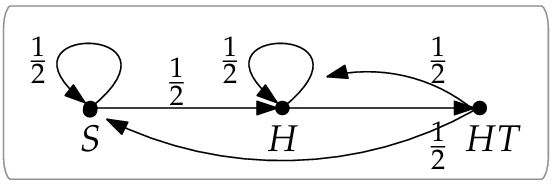
\includegraphics[scale=0.7]{images/markovchain4.PNG}
      Recurrence Time
    \end{minipage}
\end{figure}

\noindent
We know that we can quickly find the recurrence time by taking the inverse of the probability, but there also exist a shortcut to find the first passage time.
Let's take a look at the sequences $HT$ and $HH$.
These sequences are both of the same length, and thus share the same recurrence time.
However, to see $HH$ for the first time we need more flips.
In $HH$, $H$ reoccurs inside the sequence itself.
This accounts for the different \textit{starting positions} of the next sequence.
This means we need to sum the expected number of flips to see each occurrence of $H$ in the sequence:

\[ S \xrightarrow[2]{} H \xrightarrow[4]{} HH \]
\[ E_S = 6 \]

\newpage
\noindent
Let's consider the sequence $HTHTH$.
Now, without needing to draw any Markov chain, we can quickly find the recurrence time and the first passage time:

\begin{itemize}
    \item Recurrence time: $(\frac{1}{2^5})^{-1} = 32$
    \item First passage time: 42
\end{itemize}
\[ S \xrightarrow[2]{} H \xrightarrow[8]{} HTH \xrightarrow[32]{} HTHTH \]

\noindent
Some more examples include:

\[ S \xrightarrow[4]{} HT \xrightarrow[16]{} HTHT \]
\[ S \xrightarrow[2]{} H \xrightarrow[4]{} HH \xrightarrow[32]{} HHTHH \]
\[ S \xrightarrow[2]{} H \xrightarrow[32]{} HTTTH \]
\[ S \xrightarrow[2]{} H \xrightarrow[128]{} HTTTHTH \]

\subsection{Multiple Sequences}
Given two sequences of coin flips, e.g. $HTHT$ and $THHT$, which sequence do you expect to see first?
We can visualize this as the following Markov chain:

\begin{figure}[h]
    \centering
    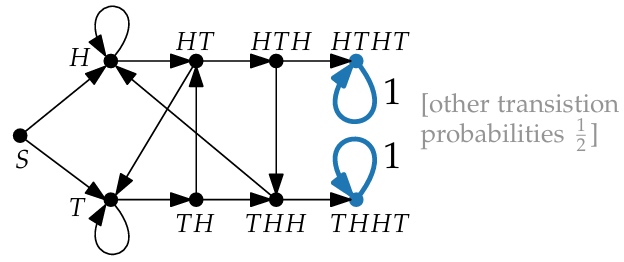
\includegraphics[scale=0.75]{images/markovchain5.PNG}
\end{figure}

\noindent
Let $P_x$ be the probability of seeing $HTHT$ before $THHT$.
We can model the Markov chain as the following system of linear equations:
\begin{equation*}
    \begin{split}
        P_S & = \frac{1}{2}P_H + \frac{1}{2}P_T \\
        P_T & = \frac{1}{2}P_T + \frac{1}{2}P_{TH} \\
        P_H & = \frac{1}{2}P_H + \frac{1}{2}P_{HT} \\
        ... & = ... \\
        P_{THHT} & = 0 \\
        P_{HTHT} & = 1
    \end{split}
\end{equation*}

\noindent
Note that, because we are now calculating probabilities, we do not need to add the 1 in front of the equations.
Since we are interested in the probability of reaching $HTHT$ before $THHT$, we manually set $P_{HTHT} = 1$ and $P_{THHT} = 0$.
If we solve the system of equations, we find that $P_S = \frac{7}{16}$, which means that on average $THHT$ will appear before $HTHT$.

%
% Topic 2 - Markov Chains
%
\newpage
\section{Markov Chains}
In addition to visual models, Markov chains can also be expressed by their \textbf{transition matrix}:

\begin{figure}[h]
    \centering
    \begin{minipage}{.5\textwidth}
      \centering
      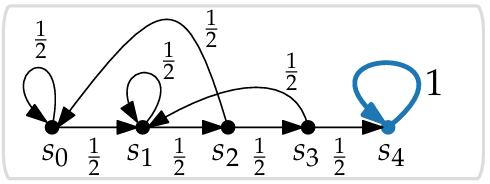
\includegraphics[scale=0.7]{images/markovchain6.PNG}
    \end{minipage}%
    \begin{minipage}{.5\textwidth}
      \centering
      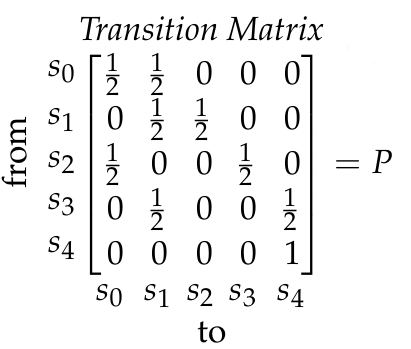
\includegraphics[scale=0.6]{images/transitionmatrix6.PNG}
    \end{minipage}
\end{figure}

\noindent
In the above example, states $s_0, s_1, s_2, s_3$ are called \textbf{transient states}.
These states are only visited finitely often.
A process starting in a transient state has by definition a non-zero probability of never returning to that state.

\noindent
\\
In the above example, state $s_4$ is a \textbf{recurrent state}.
This state is visited infinitely often.
A process starting in a recurrent state by definition will at some point return to that state.
In addition to this, $s_4$ is also an \textbf{absorbing state}.
This means that $s_4$ is inescapable.
Note that every absorbing state is also a recurrent state, but not vice-versa.
Take the following example:

\begin{figure}[h]
    \centering
    \begin{minipage}{.5\textwidth}
      \centering
      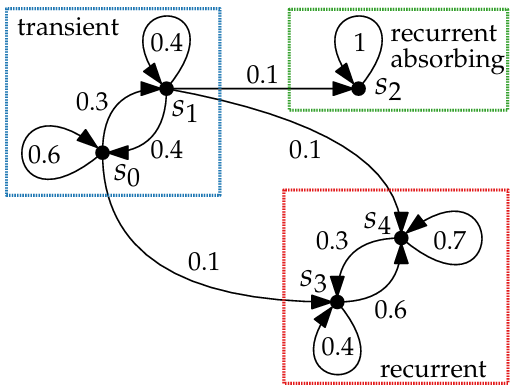
\includegraphics[scale=0.6]{images/markovchain7.PNG}
    \end{minipage}%
    \begin{minipage}{.5\textwidth}
      \centering
      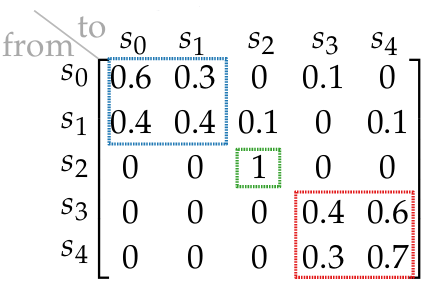
\includegraphics[scale=0.7]{images/transitionmatrix7.PNG}
    \end{minipage}
\end{figure}

\noindent
Here $s_0$ and $s_1$ are transient states.
Notice how once you leave this 'network', it is impossible to return.
$s_3$ and $s_4$ are recurrent states.
Once you end up here, it is impossible to leave to other states.
Finally, $s_2$ is both a recurrent state and an absorbing state.

\subsection{Steady-State Probabilities}
States $s_i$ and $s_j$ are said to \textbf{communicate} if there exists an $(s_i, s_j)$-path \textit{and} an $(s_j, s_i)$-path.
If all pairs of states communicate, the Markov chain is said to be \textbf{irreducible}.

\noindent
\\
Each Markov chain has a unique vector $\pi$,  where $\pi_i$ is the fraction of time spend in state $s_i$.
This is known as the \textbf{steady-state probability vector}.
If the Markov chain is irreducible, then $\pi$ has the following properties:

\begin{itemize}
    \item $\sum_{i} \pi_i = 1$ \hfill (the sum of all probabilities is 1)
    \item $\pi P = \pi$ \hfill (the probabilities are independent of the starting state)
\end{itemize}

\newpage
\noindent
Let's take the following example:

\begin{figure}[h]
    \centering
    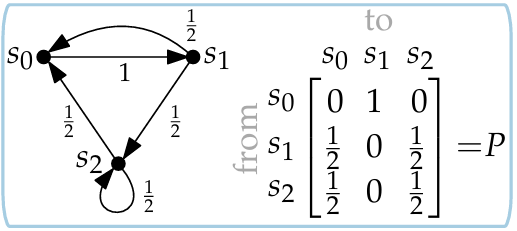
\includegraphics[scale=0.75]{images/markovchain8.PNG}
\end{figure}

\noindent
We can find the steady-state probabilities by solving the following equation:

\[ (\pi_0, \pi_1, \pi_2) = (\pi_0, \pi_1, \pi_2)\begin{bmatrix}
    0 & 1 & 0 \\
    \frac{1}{2} & 0 & \frac{1}{2} \\
    \frac{1}{2} & 0 & \frac{1}{2}
\end{bmatrix} \]

\noindent
We can write this as the following system of linear equations:

\begin{equation*}
    \systeme{
        \pi_0 = \frac{1}{2}\pi_1 + \frac{1}{2}\pi_2,
        \pi_1 = \pi_0,
        \pi_2 = \frac{1}{2}\pi_1 + \frac{1}{2}\pi_2,
        1 = \pi_0 + \pi_1 + \pi_2
    }
\end{equation*}

\noindent
Solving this system of equations, we find $\pi = \left( \frac{1}{3}, \frac{1}{3}, \frac{1}{3} \right)$.

\subsection{Periodicity}
A state is said to be \textbf{periodic} if the chain can only return to the state in multiples of some integer time step greater than 1.
The greatest common divisor of all such time steps is called the \textbf{period} of the state.
A Markov chain is (a)periodic, if all of its states are (a)periodic.
If a state is both aperiodic and recurrent, then that state is called \textbf{ergodic}.

\subsection{Short / Long Run}
We can also use the transition matrix $P$ to find the probability of being in a certain state after $t$ steps.
Let $P_{ij}^{(t)}$ be the probability of going from state $i$ to $j$ in $t$ time steps.
We can use this to calculate 'short runs' on a Markov chain, but what if we want $t$ to be infinitely large?

\noindent
\\
Let $Q$ be the $\infty$-step transition matrix, with $Q_{ij} = \displaystyle\lim_{t \to \infty} P_{ij}^t$.
If the Markov chain is aperiodic, each row $i$ of $Q$ is the steady-state probability vector $\pi$ for starting state $i$.
If the Markov chain is also irreducible, then each row of $Q$ will be the same.
This means that $Q_{ij} = \pi_j$. 

\noindent
\\
Let's revisit the second example in this chapter with the following questions:

\begin{enumerate}
    \item What is the probability of reaching state $s_2$?
    \item What is $\pi$?
    \item On average, how many times are $s_0$ and $s_1$ visited?
\end{enumerate}

\newpage
\noindent
For the first question, let $P_x$ be the probability of reaching $s_2$ starting from state $x$.
Using the transition matrix, we can create the following system of linear equations:

\begin{equation*}
    \systeme{
        P_0 = 0.6P_0 + 0.3P_1 + 0.1P_3,
        P_1 = 0.4P_0 + 0.4P_1 + 0.1P_2 + 0.1P_4,
        P_2 = 1,
        P_3 = P_4 = 0
    }
\end{equation*}

\noindent
Solving this when starting from $s_0$, we find that $P_0 = \frac{1}{4}$.

\noindent
\\
We can also use the answer from the previous question to find $\pi$.
Because $s_0$ and $s_1$ are transient states, the probability of ending up in either $s_3$ or $s_4$ is equal to $1 - \frac{1}{4} = \frac{3}{4}$.
We can find the exact probabilities similarly to what we did before:

\[ (\pi_3, \pi_4) = (\pi_3, \pi_4)\begin{bmatrix}
    0.4 & 0.6 \\
    0.3 & 0.7
\end{bmatrix} \]

\begin{equation*}
    \systeme{
        \pi_3 = 0.4\pi_3 + 0.3\pi_4,
        \pi_4 = 0.6\pi_3 + 0.7\pi_4,
        \frac{3}{4} = \pi_3 + \pi_4
    }
\end{equation*}

\noindent
Solving this, we find $\pi = \left( 0, 0, \frac{1}{4}, \frac{1}{4}, \frac{1}{2} \right)$.

\noindent
\\
To find the average visits of $s_0$ and $s_1$, we can use the following formula:

\[ S = (I - P)^{-1} \]

\noindent
Where $S_{ij}$ is the expected number of visits to state $j$ when starting from state $i$.
Since it is impossible to reach states $s_0$ and $s_1$ from other states, we can cut the transition matrix $P$ to the following:

\[ P = \begin{bmatrix}
    0.6 & 0.3 \\
    0.4 & 0.4
\end{bmatrix} \]
\[ S = \begin{bmatrix}
    S_{00} & S_{01} \\
    S_{10} & S_{11}
\end{bmatrix} = \left( I - \begin{bmatrix}
    0.6 & 0.3 \\
    0.4 & 0.4
\end{bmatrix} \right)^{-1} = \begin{bmatrix}
    5 & \frac{5}{2} \\
    \frac{10}{3} & \frac{10}{3}
\end{bmatrix} \]

\noindent
When starting in $s_0$, we can see that on average we visit $s_0$ a total of 5 times, and $s_1$ a total of $\frac{5}{2}$ times.

%
% Topic 3 - Queuing Theory
%
\newpage
\section{Queuing Theory}
Let's assume we are at a call center with the following characteristics:

\begin{itemize}
    \item The average number of calls per hour is 30.
    \item 3 agents are available to take calls, and take on average 3 minutes to handle a call.
    \item If all agents are busy, up to 2 customers can wait in line.
    \item Any other call is lost, they will have to call another time.
\end{itemize}

\noindent
We can model this system as the following Markov chain:

\begin{figure}[h]
    \centering
    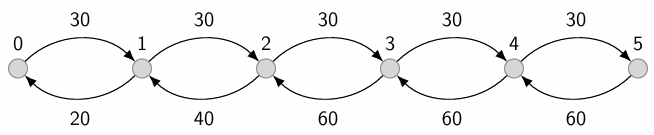
\includegraphics[scale=0.8]{images/queuingsystem1.PNG}
\end{figure}

\noindent
In this Markov chain the states represent the number of customers in the system, and the arrows represent the rate at which customers arrive / are processed.
The biggest difference between a queue and a Markov chain is that customers do not arrive and are not processed uniformly.
Instead, we deal with arrival / service times according to a probability distribution.

\subsection{Exponential Distribution}
Let $X$ be a random variable (e.g. the inter-arrival time).
$X$ is said to have an \textbf{exponential distribution} with parameter $\alpha$, if it has the following probability density function:

\begin{figure}[h]
    \centering
    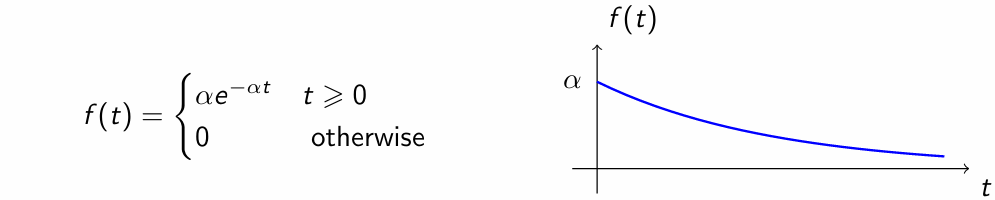
\includegraphics[scale=0.7]{images/exponentialpdf.PNG}
\end{figure}

\noindent
If customers arrive according to an exponential distribution with parameter $\alpha$, then the expected time between arrivals is $\frac{1}{\alpha}$. 
If we want to know what the probability is of an event occurring (e.g. a customer arriving) after a certain time, we can use the following formulas:
\begin{equation*}
    \begin{split}
        P[x > a] & = e^{-\alpha a} \\
        P[x \leq a] & = 1 - e^{-\alpha a} \\
        P[a < x < b] & = e^{-\alpha a} - e^{-\alpha b}
    \end{split}
\end{equation*}

\noindent
We can calculate the chance of something happening, given that something else already happened:

\[ P[x > a + c | x > c] = e^{-\alpha a} = P[x > a] \]

\noindent
This shows that the probability of a new arrival is always the same, independently of how many events there have been before.
This is called \textbf{Lack of Memory}, which links back to Markov chains selecting a future independent of the past.

\newpage
\noindent
Let $X$ and $Y$ be independent random variables with $X \sim \exp(\alpha)$ and $Y \sim \exp(\beta)$.
Let $Z = \min\{ X, Y \}$ (i.e. $Z$ is the first event among $X$ and $Y$).
We have that:
\[ Z \sim \exp(\alpha + \beta) \]

\noindent
If we want to know the probability of an event of type $X$ happening before an event of type $Y$, we can use the following formula:
\[ P[X < Y] = \frac{\alpha}{\alpha + \beta} \]

\subsection{Poisson Distribution}
Let $X \sim \exp(\alpha)$.
If we want to know the probability of $n$ events happening in $x$ time units, we model this as a \textbf{Poisson distribution} with parameter $\lambda = \alpha x$.
The probability of $n$ events happening in $x$ time units is given by the following formula:
\[ P(n \text{ events in } [0, x]) = \frac{a^n x^n}{n!}e^{-\alpha x} \]

\noindent
A Poisson process with parameter $\lambda$ models the probability of $n$ events in an interval of time when on average you would see $\lambda$ events in that given time interval.
Because of our exponential inter-arrival time, the expected number of arrivals in the time interval $[0, x]$ is $\alpha x$.

\subsection{Example}
We have call center that receives on average 30 calls per hour.
2 agents reply to calls, and can serve on average 20 calls per hour.
If all agents are busy, up to 2 customers can wait in line.
Any other call is lost.
We can model this system as the following Markov chain:

\begin{figure}[h]
    \centering
    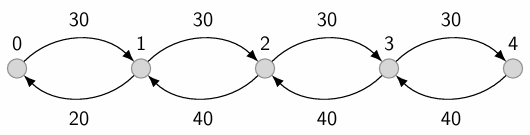
\includegraphics[scale=0.8]{images/queuingsystem2.PNG}
\end{figure}

\noindent
We are interested in the following questions:

\begin{enumerate}
    \item What fraction of time do we on average spend in each state?
    \item What is the average number of customers in the system?
    \item How much time does it on average take to go from 0 customers to 3 customers?
\end{enumerate}

\noindent
To answer the first question, let $\pi_i$ be the fraction of time spent in state $i$.
Next, we take the input and output of each state and set up the following system of linear equations:
\begin{equation*}
    \begin{split}
        20\pi_1 & = 30\pi_0 \\
        30\pi_0 + 40\pi_2 & = 20\pi_1 + 30\pi_1 \\
        30\pi_1 + 40\pi_3 & = 40\pi_2 + 30\pi_2 \\
        30\pi_2 + 40\pi_4 & = 40\pi_3 + 30\pi_3 \\
        30\pi_3 & = 40\pi_4
    \end{split}
\end{equation*}

\newpage
\noindent
If we combine this system of equations with the fact that the sum of all probabilities is 1, we can solve this system of equations to find:
\[ \pi = \frac{1}{653} \left( 128, 192, 144, 108, 81 \right) \]

\noindent
To get the average number of customers in the system, we can simply multiply $\pi$ with the number of customers in each state:
\[ 0 \cdot \pi_0 + 1 \cdot \pi_1 + 2 \cdot \pi_2 + 3 \cdot \pi_3 + 4 \cdot \pi_4 \approx 1.7 \]

\noindent
The last question is to find the average time to go from 0 to 3 customers.
Let $E_x$ be the expected time to go from state $x$ to state 3.
This is equal to the expected time spent in state $x$ plus the sum of transition probabilities to other states times the expected time to go from that state to state 3:
\[ E_x = \text{ Time in } x + \sum P_{xi}E_{i} \]

\noindent
To get the time spent in state $x$, we can look at the rate at which we leave the state:

\begin{itemize}
    \item State 0: 30 events per hour leave to state 1, so the time per visit is $\frac{1}{30}$ hours.
    \item State 1: 20 + 30 events per hour leave, so the time per visit is $\frac{1}{50}$ hours.
    \item State 2: 30 + 40 events per hour leave, so the time per visit is $\frac{1}{70}$ hours.
    \item State 4: 40 events per hour leave to state 3, so the time per visit is $\frac{1}{40}$ hours.
\end{itemize}

\noindent
We can now set up the following system of linear equations:
\begin{equation*}
    \begin{split}
        E_0 & = \frac{1}{30} + E_1 \\
        E_1 & = \frac{1}{50} + \frac{2}{5}E_0 + \frac{3}{5}E_2 \\
        E_2 & = \frac{1}{70} + \frac{4}{7}E_1 + \frac{3}{7}E_3 \\
        E_3 & = 0
    \end{split}
\end{equation*}

\noindent
Solving this system of equations, we find that $E_0 = \frac{53}{270}$.

%
% Topic 4 - Markov Decision Processes
%
\newpage
\section{Markov Decision Processes}
Let's consider the following example:
A manufacturer has a machine at the center of its production process.
After some time the machine might deteriorate, hence it has to be regularly checked.
The machine can be in the following states:

\begin{enumerate}\addtocounter{enumi}{-1}
    \item Good as new.
    \item Operable, minor defects.
    \item Operable, major defects, needs repair.
    \item Inoperable, needs replacement.
\end{enumerate}

\noindent
These states can change according to the following transition matrix:
\[ P = \begin{bmatrix}
    0 & \frac{7}{8} & \frac{1}{16} & \frac{1}{16} \\
    0 & \frac{3}{4} & \frac{1}{8} & \frac{1}{8} \\
    0 & 0 & \frac{1}{2} & \frac{1}{2} \\
    1 & 0 & 0 & 0
\end{bmatrix} \]

\noindent
Depending on the state of the machine, the manufacturer can take the following actions:

\begin{enumerate}
    \item Do nothing.
    \item Repair (only possible in state 2).
    \item Replace.
\end{enumerate}

\noindent
However, the manufacturer has to pay for these actions.
Repairing the machine costs 4000, and buying a new one costs 6000.
Additionally, continuing to use the machine in state 1 or 2 costs 1000 and 3000 per time step respectively.

\noindent
\\
We can summarize all this information in the following model:

\begin{figure}[h]
    \centering
    \begin{minipage}{.25\textwidth}
      \centering
      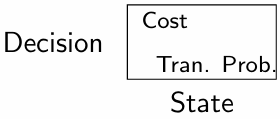
\includegraphics[scale=0.65]{images/markovdecisionprocess1.PNG}
    \end{minipage}%
    \begin{minipage}{.7\textwidth}
      \centering
      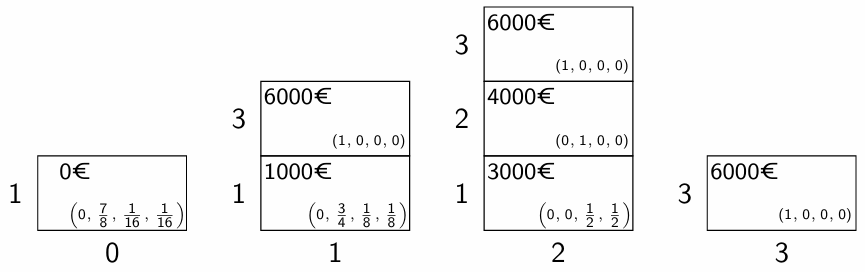
\includegraphics[scale=0.6]{images/markovdecisionprocess2.PNG}
    \end{minipage}
\end{figure}

\noindent
Note that the transition matrix $P$ corresponds to the probabilities of the bottom row.
It is said that the transition matrix $P$ corresponds to the \textbf{policy} $(1, 1, 1, 3)$.
This means that the manufacturer makes decision 1 in state 0, 1 in state 1, 1 in state 2, and 3 in state 3.
If we want to find the transition matrix for a different policy, for example $(1, 3, 2, 3)$, we can construct it in the same way:

\[ P = \begin{bmatrix}
    0 & \frac{7}{8} & \frac{1}{16} & \frac{1}{16} \\
    1 & 0 & 0 & 0 \\
    0 & 1 & 0 & 0 \\
    1 & 0 & 0 & 0
\end{bmatrix} \]

\newpage
\subsection{Minimizing Cost}
The goal of a Markov decision process is to find the policy that minimizes the cost.
To do this we compute the \textbf{expected average cost} (per unit time) for all possible policies.

\noindent
\\
To calculate the expected average cost for a policy, we calculate the time spent in each state (the steady-state probabilities) and multiply this with the cost of being in that state.
Doing this for all policies in the example, we find the following expected average costs:

\begin{table}[h]
    \centering
    \begin{tabular}{c|c}
    Policy & Cost \\ \hline
    $(1, 1, 1, 3)$ & 1923 \\
    $(1, 1, 2, 3)$ & 1666 \\
    $(1, 1, 3, 3)$ & 1727 \\
    $(1, 3, 1, 3)$ & 3000 \\
    $(1, 3, 2, 3)$ & 3030 \\
    $(1, 3, 3, 3)$ & 3000
    \end{tabular}
\end{table}

\noindent
From this we can conclude that $(1, 1, 2, 3)$ is the cheapest policy.

\noindent
\\
Note that to find the optimal policy, we need to calculate the expected average cost for all possible policies.
This is not feasible for large Markov decision processes.
One faster way to find the optimal policy is to use \textbf{linear programming}.
Let $y_{ik}$ be the probability of taking action $k$ in state $i$.
We can model the minimum cost problem as the following linear program:
\begin{align*}
    &\mathrm{min} \quad \sum_{i}\sum_{k} y_{ik} C_{ik} \\[2pt]
    &\mathrm{s.t.} \quad 
    \begin{array}[t]{r c l l}
        \displaystyle\sum_{i}\displaystyle\sum_{k} y_{ik} & = & 1 & \\
        \displaystyle\sum_{k} y_{jk} & = & \displaystyle\sum_{i}\displaystyle\sum_{k} y_{ik} P_{ij}(k) & \forall j \\
        y_{ik} & \geq & 0 & \forall i \forall k
     \end{array}
\end{align*}

\noindent
Here $C_{ik}$ is the cost of taking action $k$ in state $i$, and $P_{ij}(k)$ is the probability of going from state $i$ to state $j$ when taking action $k$.
The first constraint ensures that the sum of all probabilities is 1.
The second constraint says that the sum of all actions in state $j$ is equal to the sum of all actions leading to state $j$ times to probability of those actions occurring.
Filling in the costs and probabilities for the example, we can construct the following linear program:
\begin{align*}
    &\mathrm{min} \quad 0y_{01} + 1000y_{11} + 6000y_{13} + 3000y_{21} + 4000y_{22} + 6000y_{23} + 6000y_{33} \\[2pt]
    &\mathrm{s.t.} \quad 
    \begin{array}[t]{r c l l}
        y_{01} + y_{11} + y_{13} + y_{21} + y_{22} + y_{23} + y_{33} & = & 1 & \\
        y_{01} & = & y_{13} + y_{23} + y_{33} & \\
        y_{11} + y_{13} & = & \frac{7}{8}y_{01} + \frac{3}{4}y_{11} + y_{22} & \\
        y_{21} + y_{22} + y_{23} & = & \frac{1}{16}y_{01} + \frac{1}{8}y_{11} + \frac{1}{2}y_{21} & \\
        y_{33} & = & \frac{1}{16}y_{01} + \frac{1}{8}y_{11} + \frac{1}{2}y_{21} & \\
        y_{ik} & \geq & 0 & \forall i \forall k
     \end{array}
\end{align*}

\newpage
\subsection{Discounted Markov Decision Processes}
Let $\alpha \in [0, 1]$ be the effect of future costs on the decision we make today.
This is called the \textbf{discount factor}.
A value of $\alpha = 0$ means that more importance is given to the present, and a value of $\alpha = 1$ means that more importance is given to the future.
For example, the discount factor could be the interest rates: $\alpha = \frac{1}{1 + i}$.
Implicitly, we assume that the process is going to end at any point in time with probability $1 - \alpha$.

\subsubsection{Discounted Number of Visits}
As an example, consider the following Markov chain:

\begin{figure}[h]
    \centering
    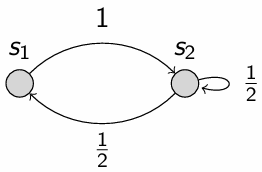
\includegraphics[scale=0.8]{images/markovchain9.PNG}
\end{figure}

\noindent
Let $\delta_i$ be the \textbf{discounted number of visits} to state $i$ (i.e. the probability of being there + the probability of coming there).
Using the discount factor $\alpha$, we can construct the following equations:
\[ \delta_1 = \frac{1}{2} + \alpha \frac{1}{2}\delta_2 \]
\[ \delta_2 = \frac{1}{2} + \alpha \left( \delta_1 + \frac{1}{2}\delta_2 \right) \]

\noindent
By combining these equations we can find that, on average, the process ends after $\delta_1 + \delta_2 = \frac{1}{1 - \alpha}$ steps.
Another way to see this is to use the assumption that the process ends at any point in time with probability $1 - \alpha$, which is like going to an absorbing state with probability $1 - \alpha$:

\begin{figure}[h]
    \centering
    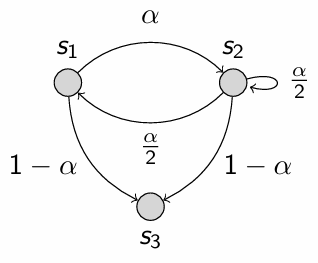
\includegraphics[scale=0.75]{images/markovchain10.PNG}
\end{figure}

\noindent
If we calculate the expected number of visits to state 1 and 2, we also find $\frac{1}{1 - \alpha}$, which verifies our assumption.

\subsubsection{Discounted Cost}
Let us include some costs in the previous Markov chain.
In state 1 we have a cost of 1, and in state 2 we have a cost of 2.
Let $\delta_i$ be the \textbf{discounted cost} of being in state $i$ (i.e. what we have to pay here + what we have to pay if we move):

\newpage
\[ \delta_1 = \alpha \frac{1}{2}\delta_2 \]
\[ \delta_2 = 2 + \alpha \left( \delta_1 + \frac{1}{2}\delta_2 \right) \]

\noindent
Solving these equations, we find the following expected costs:
\[ \delta_1 = \frac{2 + 3\alpha}{(1 - \alpha)(\alpha + 2)} \]
\[ \delta_2 = \frac{4 + \alpha}{(1 - \alpha)(\alpha + 2)} \]

\noindent
If $\alpha \rightarrow 1$ (i.e. we look infinitely far into the future), then $\delta_1, \delta_2 \rightarrow \infty$.
We can also take a look at the \textbf{normalized discount costs}:
\[ (1 - \alpha)\delta_1 = \frac{2 + 3\alpha}{\alpha + 2} \]
\[ (1 - \alpha)\delta_2 = \frac{4 + \alpha}{\alpha + 2} \]

\noindent
If $\alpha \rightarrow 1$, then both normalized costs converge to $\frac{5}{3}$, the \textbf{average cost} obtained by multiplying the costs by the time spent per state.

\subsubsection{Discounted Linear Program}
Similarly to a regular Markov decision process, we can use linear programming to find the optimal policy for a discounted Markov decision process.
This linear program looks like this:
\begin{align*}
    &\mathrm{min} \quad \sum_{i}\sum_{k} y_{ik} C_{ik} \\[2pt]
    &\mathrm{s.t.} \quad 
    \begin{array}[t]{r c l l}
        \displaystyle\sum_{k} y_{jk} & = & \displaystyle\frac{1}{z} + \alpha \displaystyle\sum_{i}\displaystyle\sum_{k} y_{ik} P_{ij}(k) & \forall j \\
        y_{ik} & \geq & 0 & \forall i \forall k
     \end{array}
\end{align*}

\noindent
Where $z$ is the number of states.
The big difference here is that $y_{ik}$ is now the expected number of times that action $k$ is chosen while in state $i$.
This means that $y_{ik}$ is no longer a probability, and also does not sum up to 1 anymore:
\[ \sum_i \sum_k y_{ik} = \frac{1}{1 - \alpha} \]

\noindent
Taking the example used in the previous section, we can construct the following linear program:
\begin{align*}
    &\mathrm{min} \quad 0y_{01} + 1000y_{11} + 6000y_{13} + 3000y_{21} + 4000y_{22} + 6000y_{23} + 6000y_{33} \\[2pt]
    &\mathrm{s.t.} \quad 
    \begin{array}[t]{r c l l}
        y_{01} & = & \frac{1}{4} + \alpha (y_{13} + y_{23} + y_{33}) & \\
        y_{11} + y_{13} & = & \frac{1}{4} + \alpha (\frac{7}{8}y_{01} + \frac{3}{4}y_{11} + y_{22}) & \\
        y_{21} + y_{22} + y_{23} & = & \frac{1}{4} + \alpha (\frac{1}{16}y_{01} + \frac{1}{8}y_{11} + \frac{1}{2}y_{21}) & \\
        y_{33} & = & \frac{1}{4} + \alpha (\frac{1}{16}y_{01} + \frac{1}{8}y_{11} + \frac{1}{2}y_{21}) & \\
        y_{ik} & \geq & 0 & \forall i \forall k
     \end{array}
\end{align*}

%
% Topic 5 - Transportation Problems
%
\newpage
\section{Transportation Problems}
One of the main products of the P \& T Company is canned peas.
These peas are prepared at three canneries, and then shipped by truck to four warehouses.
Because shipping costs are expensive, the company wants to find the cheapest way to distribute the peas.
Information about the shipping costs, the space available at the warehouses, and the output of the canneries is given in the following table:

\begin{figure}[h]
    \centering
    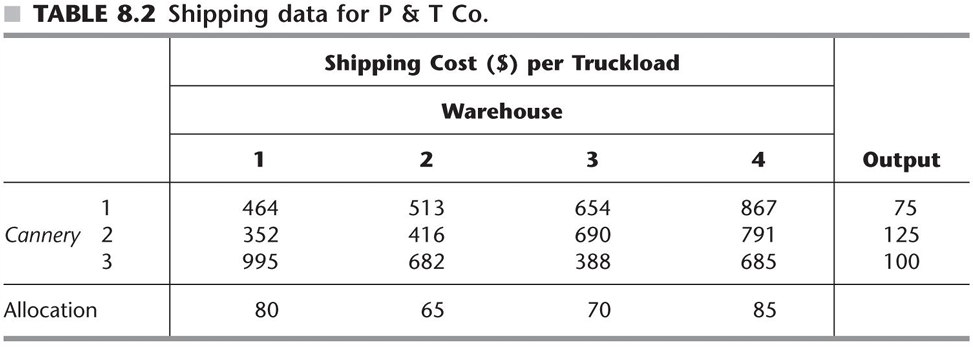
\includegraphics[scale=0.675]{images/transportationproblem1.PNG}
\end{figure}

\noindent
We can also create a \textbf{network representation} of this problem:

\begin{figure}[h]
    \centering
    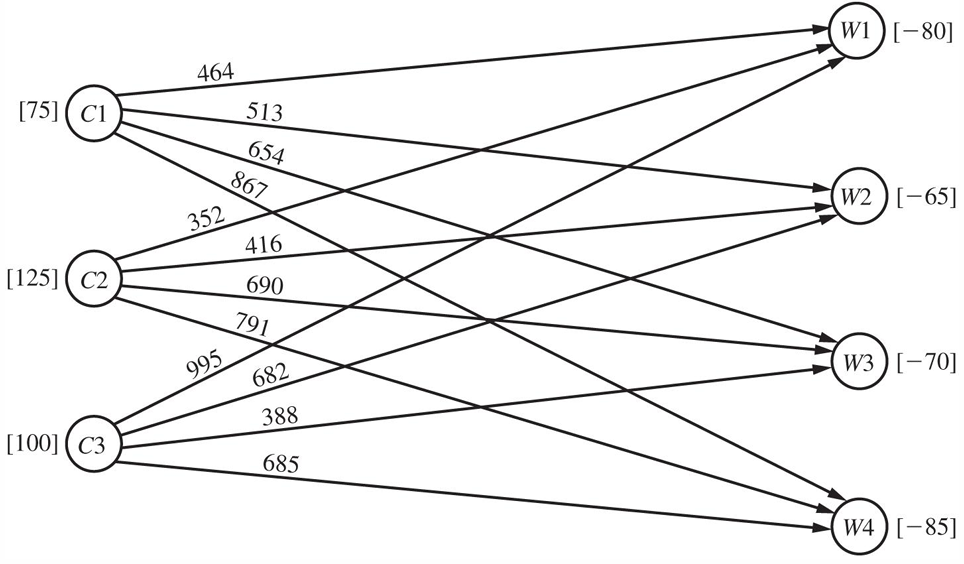
\includegraphics[scale=0.55]{images/transportationproblem2.PNG}
\end{figure}

\noindent
If we let $x_{ij}$ be the amount of truckloads shipped from cannery $i$ to warehouse $j$, we can also model this problem as a linear program.
In tabular form, this linear program has the following constraint coefficients:

\begin{figure}[h!]
    \centering
    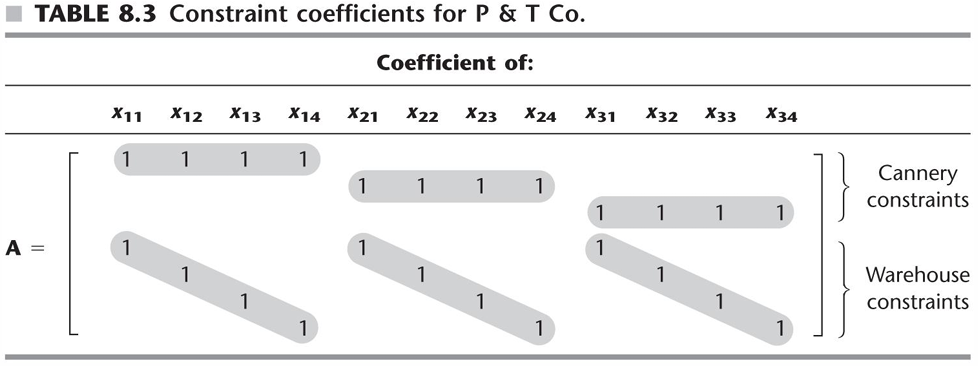
\includegraphics[scale=0.675]{images/transportationproblem3.PNG}
\end{figure}

\newpage
\noindent
It is the special structure of these constraint coefficients that makes this problem a \textbf{transportation problem}, not the context.
In general, a transportation problem is concerned with distributing any goods from any number of supply centers, called \textbf{sources}, to any group of receiving centers, called \textbf{destinations}, in such a way as to minimize the total distribution costs:

\begin{figure}[h]
    \centering
    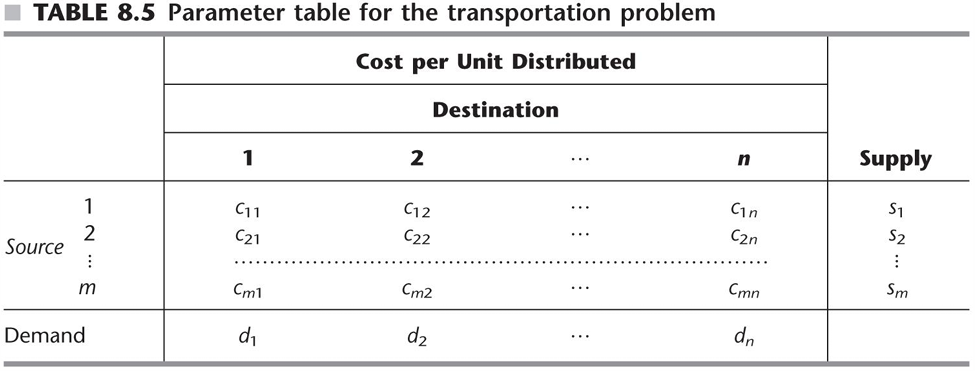
\includegraphics[scale=0.65]{images/transportationproblem4.PNG}
\end{figure}

\noindent
Note that for any feasible solutions to exist, the total supply must equal the total demand.
Furthermore, every transportation problem has constraint coefficients in the following form:

\begin{figure}[h]
    \centering
    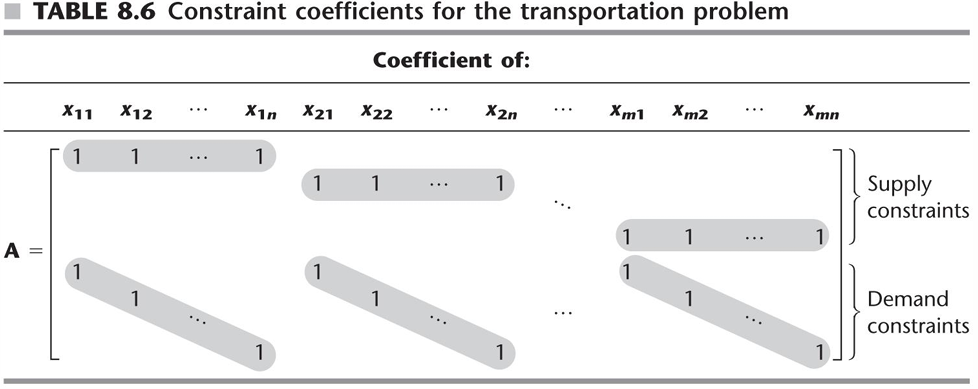
\includegraphics[scale=0.6]{images/transportationproblem5.PNG}
\end{figure}

\subsection{Modelling Transportation Problems}
In some real world problems, the supply actually represents the maximum amount that can be shipped from the source (instead of a fixed amount).
This would not fit as a transportation problem, since the supply and demand are not strictly equal.
However, it is possible to transform this problem into a transportation problem by adding a \textbf{dummy destination} or a \textbf{dummy source}, to take up the slack between the maximum and actual amounts being distributed.
Take the following example:

\begin{figure}[h]
    \centering
    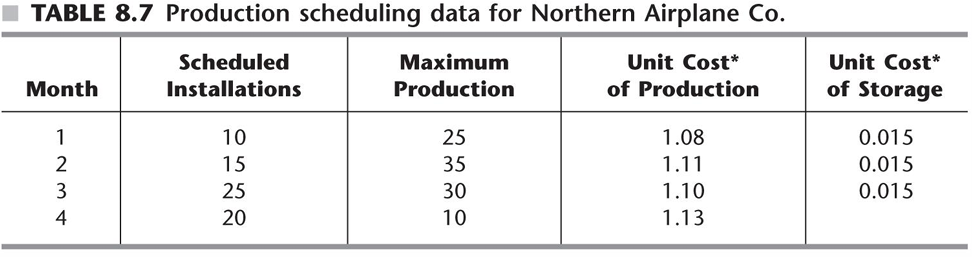
\includegraphics[scale=0.7]{images/transportationproblem6.PNG}
\end{figure}

\newpage
\noindent
To save money, an airplane company is considering producing engines in advance that will only be fit in a later month.
Each month has a scheduled number of installations, a maximum number of engines that can be produced, a production cost, and a storage cost.
The company wants to find the cheapest way to produce the engines.
We can model this as the following transportation problem:

\begin{figure}[h]
    \centering
    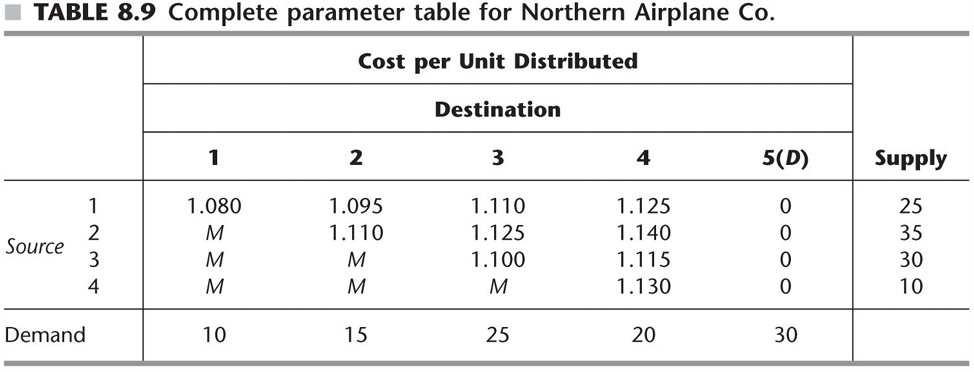
\includegraphics[scale=0.6]{images/transportationproblem7.PNG}
\end{figure}

\noindent
Here the source and destination are the months, and the cost per unit is calculated as the production cost plus the total storage cost.
The \textbf{Big M} method can be used to prevent the production of engines for months in the past, and we use a \textbf{dummy destination} to take up the slack between the maximum and actual amounts being produced.

\noindent
\\
An additional property of transportation problems is that, if the supplies and demands are all integers, then there will always exist an integer optimal solution.

\noindent
\\
As one final example, consider the following problem:
We want to supply four cities (Berdoo, Los Devils, San Go, Hollyglass) with water from three rivers (Hollyglass cannot be supplied from Calorie River).
Each river has a fixed capacity, and each city has a minimum and maximum demand:

\begin{figure}[h]
    \centering
    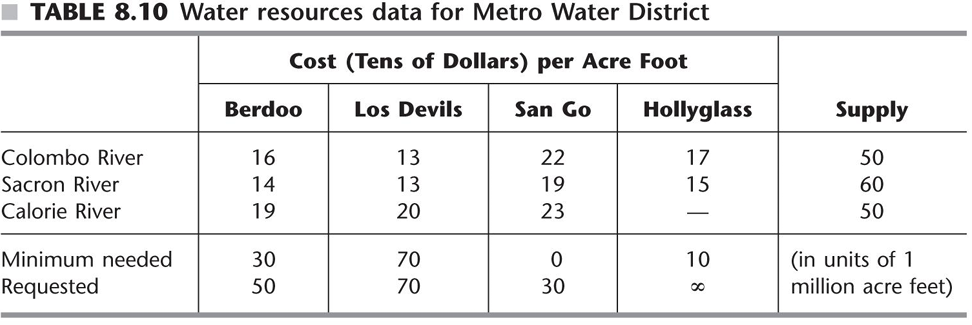
\includegraphics[scale=0.7]{images/transportationproblem8.PNG}
\end{figure}

\noindent
How do we model this as a transportation problem?
First, we replace the dash for Hollyglass and Calorie River with an $M$.
Hollyglass has a maximum demand of $\infty$, but we can calculate that this upper bound is in practice only equal to $(50 + 60 + 50) - (30 + 70 + 0) = 60$.
To account for the upper bound, we also add a \textbf{dummy source} to account for the slack between the maximum and actual amounts being distributed:

\newpage
\begin{figure}[h!]
    \centering
    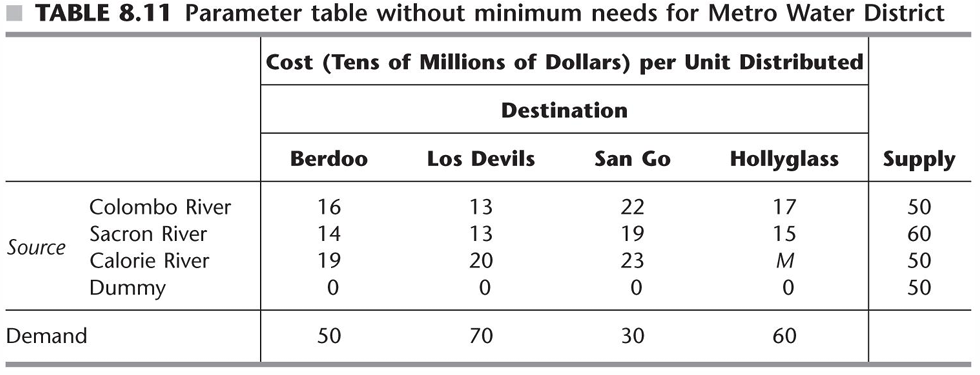
\includegraphics[scale=0.65]{images/transportationproblem9.PNG}
\end{figure}

\noindent
The only thing left to do is to account for the minimum demands.
Since San Go has a minimum demand of 0, we can leave it alone.
Los Devils has the same minimum and maximum demand, so we can replace its dummy value with an $M$ to prevent it taking any dummy water.
In Hollyglass, we don't need to do anything.
The difference between the minimum and maximum demand of Hollyglass is 50, which is also the maximum amount of dummy water that can be taken.
Finally, Berdoo requires some more attention.
We split Berdoo into two destinations.
One destination has the minimum demand of 30 and is not allowed to take any slack, while the second destination has a demand of $50 - 30 = 20$, while allowing slack:

\begin{figure}[h]
    \centering
    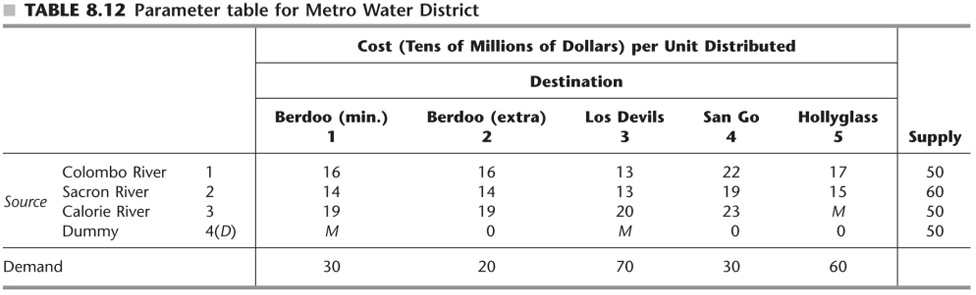
\includegraphics[scale=0.75]{images/transportationproblem10.PNG}
\end{figure}

\subsection{The Transportation Simplex Method}
Conceptually, the \textbf{Transportation Simplex Method} is very similar to the general Simplex method:

\begin{enumerate}
    \item Construct an initial basic feasible solution (BFS).
    \item Check whether the current BFS is optimal.
    \item If not, identify the nonbasic variable with the most potential to improve the objective function (the entering variable, this will swap from nonbasic to basic), and identify the variable in the current basis that will leave when the entering variable enters (leaving variables, this will swap from basic to nonbasic).
\end{enumerate}

\noindent
Remember that \textbf{nonbasic variables} are variables that are forced to be 0, while \textbf{basic variables} are variables that are potentially non-zero.
The basic variables carry the unique solution to the system of equalities after the nonbasic variables have been set to 0.
An interesting property of the transportation Simplex method is that there will \textit{always} be $(m + n - 1)$ basic variables.

\newpage
\noindent
Fortunately, the transportation problem has a special structure that makes the Simplex method much easier.
We will use the water district example to illustrate this.

\subsubsection{Initial Basic Feasible Solution}
The simplest way to construct an initial BFS to a transportation problem is to use the \textbf{Northwest Corner Rule}:

\begin{figure}[h]
    \centering
    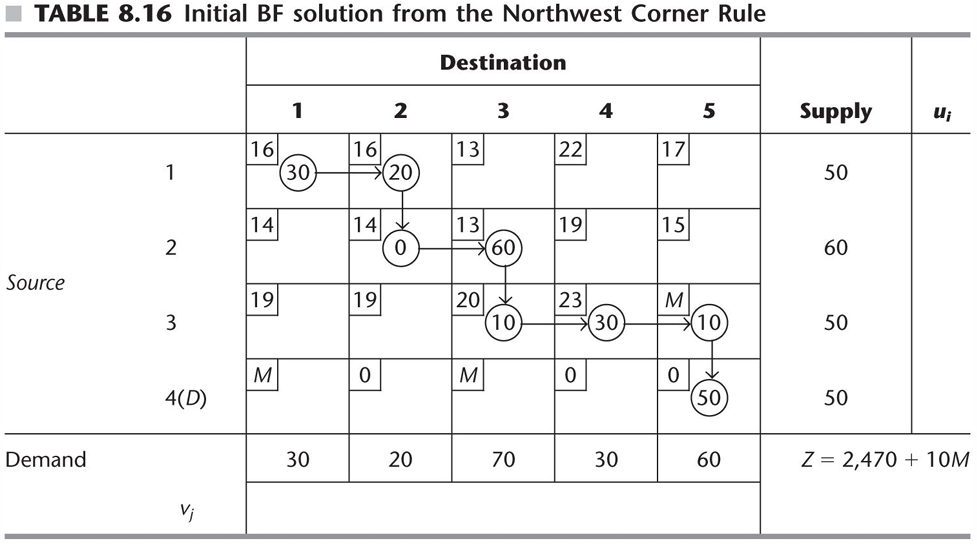
\includegraphics[scale=0.65]{images/northwestcornerrule.PNG}
\end{figure}

\noindent
This rule starts in the top-left corner of the tableau, and fills in the cells by moving to the right or down.
The first cell is filled with the minimum of the supply and demand.
The supply or demand is then reduced by this amount, and we try to move to the right.
If we do not have enough supply to reach the current demand, we move down instead.
This process is repeated until all demand has been met.
The circled numbers in the above image represent the \textbf{initial BFS}.

\noindent
\\
Note that the above image also illustrates the proper tableau structure for a transportation problem, including the $v_j$, $u_i$ and $Z$ variables.
The initial value of $Z$ is calculated by summing the costs of the filled cells, multiplied by the amount in each cell.

\subsubsection{Optimality Check}
In the general Simplex method we can determine whether the current BFS is optimal by looking at the top row of the Simplex tableau.
If all coefficients are positive, then the current BFS is optimal.
Exactly the same idea works with the transportation Simplex method, the difference is that we can do this more quickly.
To check whether the current BFS is optimal, we need to fill in the remaining cells of the tableau.
If none of the values are negative, then the current BFS is optimal.
The missing values can be filled in using the following formula:
\[ \text{value}_{ij} = c_{ij} - u_i - v_j \]

\noindent
We already have $c_{ij}$ from the original problem, but we still need to calculate $u_i$ and $v_j$.
Fortunately, these can be derived from the current BFS.
For the $(m + n - 1)$ basic variables, the equation $c_{ij} - u_i - v_j = 0$ holds.
This means that we can obtain $(m + n - 1)$ equations with $(m + n)$ unknowns.
We can solve this system of equations by arbitrarily setting one of the $u_i$ and $v_j$ values to 0, which gives us enough information to fill in all the missing values.

\newpage
\subsubsection{Pivoting}
Just like the normal Simplex method, we select the nonbasic variable with the most negative value as the entering variable.
To find the leaving variable, we need to look at the \textbf{closed loop} created by the entering variable.
After filling in the values in the example, we end up with the following tableau:

\begin{figure}[h]
    \centering
    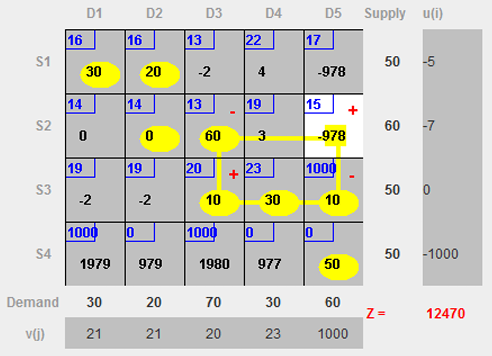
\includegraphics[scale=0.75]{images/transportationsimplex1.PNG}
\end{figure}

\noindent
We select $(S_2, D_5)$ as the entering variable.
This means that we will (potentially) increase the amount of water shipped from source 2 to destination 5.
To keep the constraints satisfied, we need to decrease the amount of water shipped from source 2 to destination 3.
This in turn means that we need to increase the amount of water shipped from source 3 to destination 3 (to keep the demand constraint satisfied).
Finally, we need to decrease the amount of water shipped from source 3 to destination 5 (to keep the supply constraint satisfied).
This one change to $(S_2, D_5)$ creates a \textbf{closed loop} of changes to the basic variables.
These changes are indicated in the tableau with a $+$ or $-$ sign.

\noindent
\\
Since $(S_3, D_5)$ is the decreasing basic variable with the lowest value, this will become the leaving variable.
The entering value will take the value of the leaving value, and the leaving value will take the value of the entering value, but positive.
The rest of the basic variables will be updated according to the closed loop:

\begin{figure}[h]
    \centering
    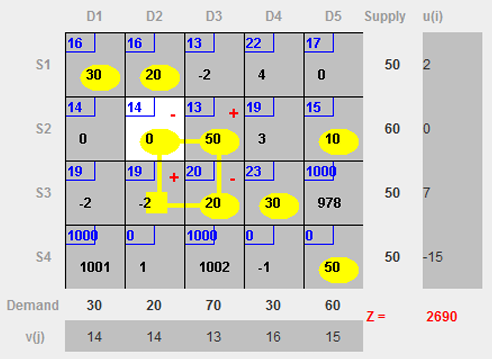
\includegraphics[scale=0.75]{images/transportationsimplex2.PNG}
\end{figure}

\noindent
Next, we are going to make $(S_3, D_2)$ basic.
This is going to be a \textbf{degenerate pivot}, since the leaving variable has a value of 0.
This also means that the $Z$ value is not going to change.

\newpage
\noindent
The remaining pivots are as follows:

\begin{figure}[h]
    \centering
    \begin{minipage}{.5\textwidth}
      \centering
      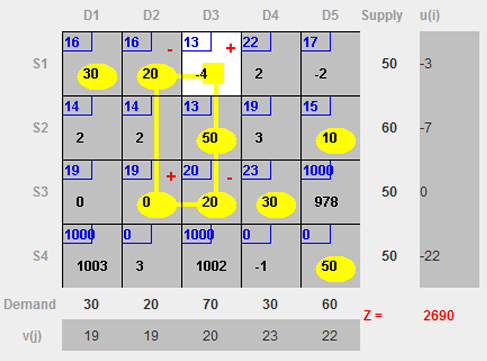
\includegraphics[scale=0.7]{images/transportationsimplex3.PNG}
      \\entering: $(S_1, D_3)$, leaving: $(S_3, D_3)$
    \end{minipage}%
    \begin{minipage}{.5\textwidth}
      \centering
      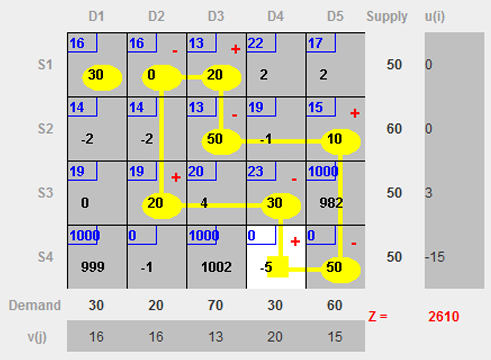
\includegraphics[scale=0.7]{images/transportationsimplex4.PNG}
      \\entering: $(S_4, D_4)$, leaving: $(S_1, D_2)$ (degen.)
    \end{minipage}
\end{figure}

\begin{figure}[h]
    \centering
    \begin{minipage}{.5\textwidth}
      \centering
      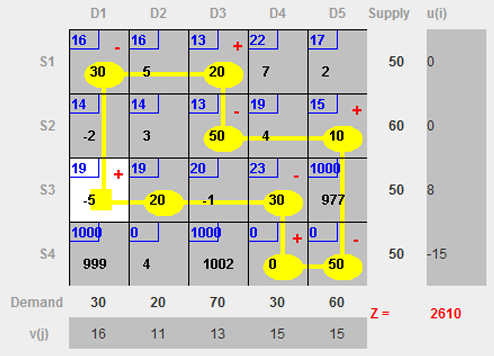
\includegraphics[scale=0.7]{images/transportationsimplex5.PNG}
      \\entering: $(S_3, D_1)$, leaving: $(S_3, D_4)$
    \end{minipage}%
    \begin{minipage}{.5\textwidth}
      \centering
      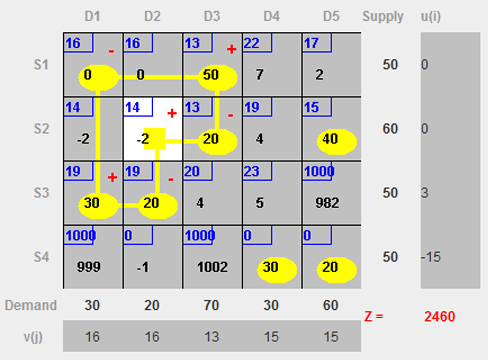
\includegraphics[scale=0.7]{images/transportationsimplex6.PNG}
      \\entering: $(S_2, D_2)$, leaving: $(S_1, D_1)$ (degen.)
    \end{minipage}
\end{figure}

\noindent
After the final pivot, there are no more negative values in the gray squares.
The optimal cost is $Z = 2460$, and the values of the basic variables can be found in the yellow circles.

\subsection{The Assignment Problem}
The \textbf{Assignment Problem} is a special case of the transportation problem.
In the assignment problem, we have $n$ workers and $n$ tasks.
Each worker can only be assigned to one task, and each task can only be assigned to one worker.
Each worker has different skills, so the time required to complete a task changes from worker to worker.
The goal is to find the optimal assignment of workers to tasks, such that the total time required is minimized.

\noindent
\\
This can be modelled as a transportation problem where each worker has a supply of 1, each task has a demand of 1, and $c_{ij}$ is the time required for worker $i$ to complete task $j$.
Through the integrality property of the transportation problem, we know that there will always exist an integer optimal solution that models a legitimate assignment of workers to tasks.

%
% Topic 6 - Flow Networks
%
\newpage
\section{Flow Networks}
Many famous graph problems can be modelled as special cases of the \textbf{minimum-cost flow problem}, which can be solved using the \textbf{network Simplex method}.
Examples of such problems include the maximum flow problem, the shortest path problem, and the transportation problem.

\subsection{Minimum-Cost Flow Problem}
The minimum-cost flow problem asks what the cheapest way is to send a certain amount of flow from a set of supply points to a set of demand points.
Arcs in the network have a cost per unit of flow, as well as a maximum capacity.
As usual in flow networks, the total flow into a node must equal the total flow out of a node (except for supply and demand nodes).

\noindent
\\
The minimum-cost flow problem acts as a generalization of problems like the maximum flow problem and the shortest path problem.
It is interesting to study this problem because it can be solved using the network Simplex method, which can solve minimum-cost flow problems up to 100 times faster than the general Simplex method.

\noindent
\\
Minimum-cost flow problems are usually given in the following form:

\begin{figure}[h]
    \centering
    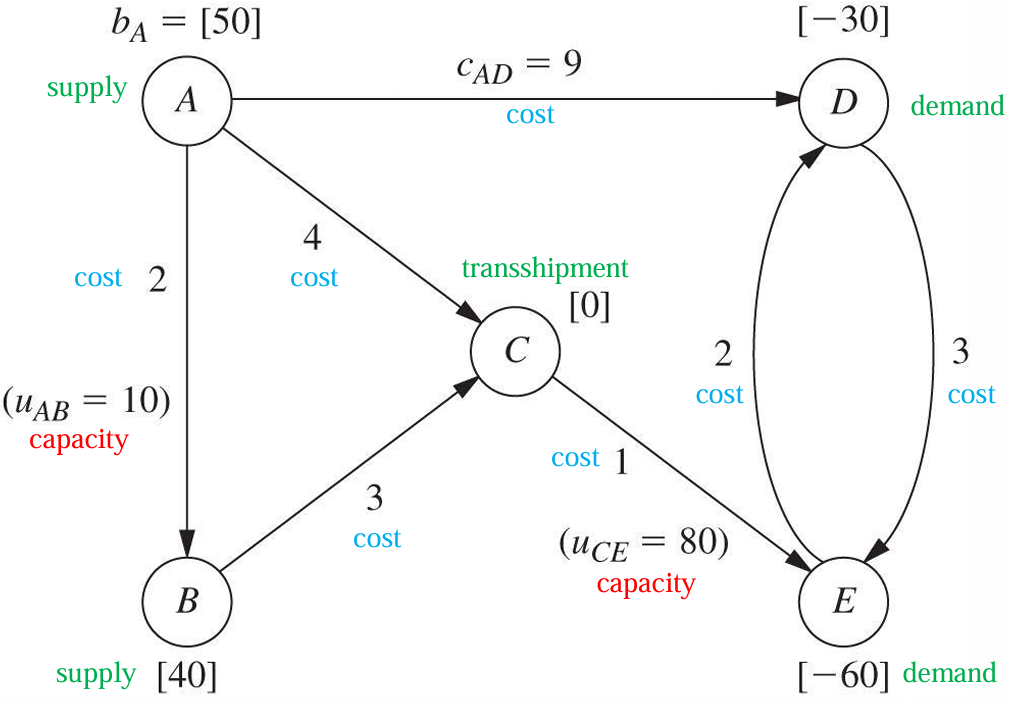
\includegraphics[scale=0.6]{images/flownetwork1.PNG}
\end{figure}

\noindent
In most example problems, the total supply is equal to the total demand.
If this is not the case, we can always add \textbf{dummy nodes} to the network to balance the supply and demand.
Similarly to the transportation problem, if all arc capacities, supplies and demands are integers, then every basic feasible solution will also be integral.

\noindent
\\
The minimum-cost flow problem can be modelled as a linear program.
The high-level structure of this linear program is as follows:
Minimize the total cost of the flow, subject to the constraints that the flow into a node equals the flow out of a node, and that the flow on each arc is between 0 and the capacity of that arc.

\newpage
\subsection{Modelling Flow Networks}
In this section we will show some examples of problems being modelled as minimum-cost flow problems.

\subsubsection{The Transportation Problem}

\begin{figure}[h]
    \centering
    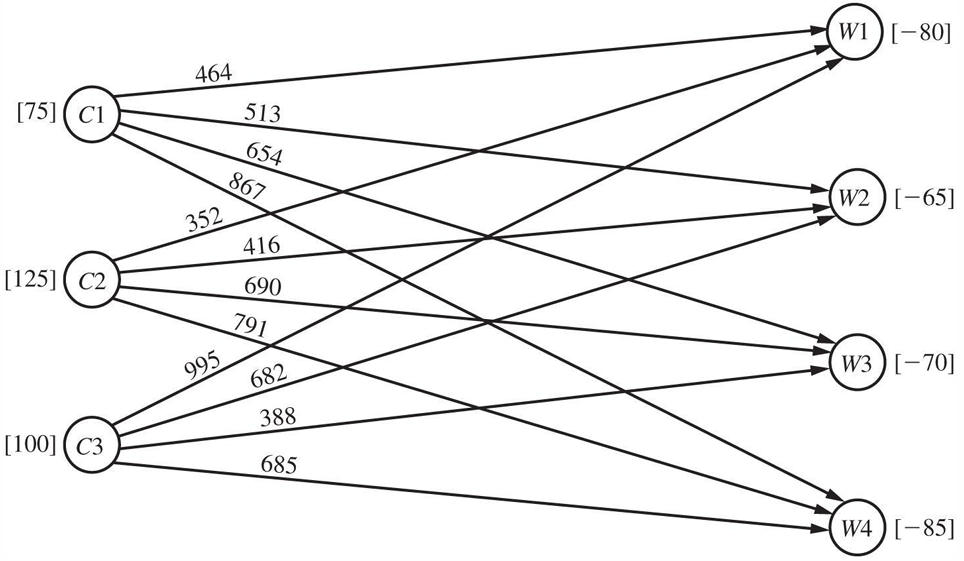
\includegraphics[scale=0.7]{images/flownetwork2.PNG}
\end{figure}

\noindent
When modelling the transportation problem as a minimum-cost flow problem, we connect all supply nodes to all demand nodes (with no transshipment nodes) with infinite flow capacities.

\subsubsection{The Shortest Path Problem}

\begin{figure}[h]
    \centering
    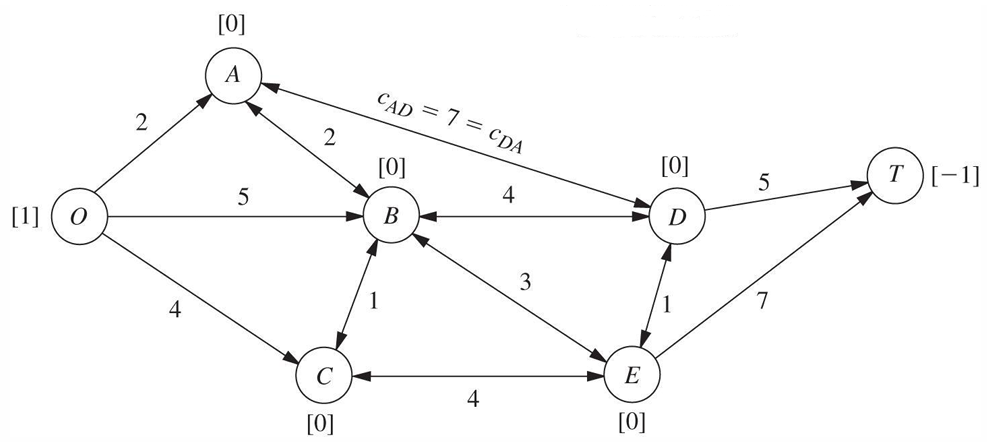
\includegraphics[scale=0.7]{images/flownetwork3.PNG}
\end{figure}

\noindent
For the shortest path problem, we use only a single supply node generating 1 unit of flow, and a single demand node consuming 1 unit of flow.
There are no arc capacities, and the cost of each arc is equal to the distance between the nodes.
Undirected edges can be modelled as two directed arcs with the same cost (as seen in the example above).

\newpage
\subsubsection{The Maximum Flow Problem}

\begin{figure}[h]
    \centering
    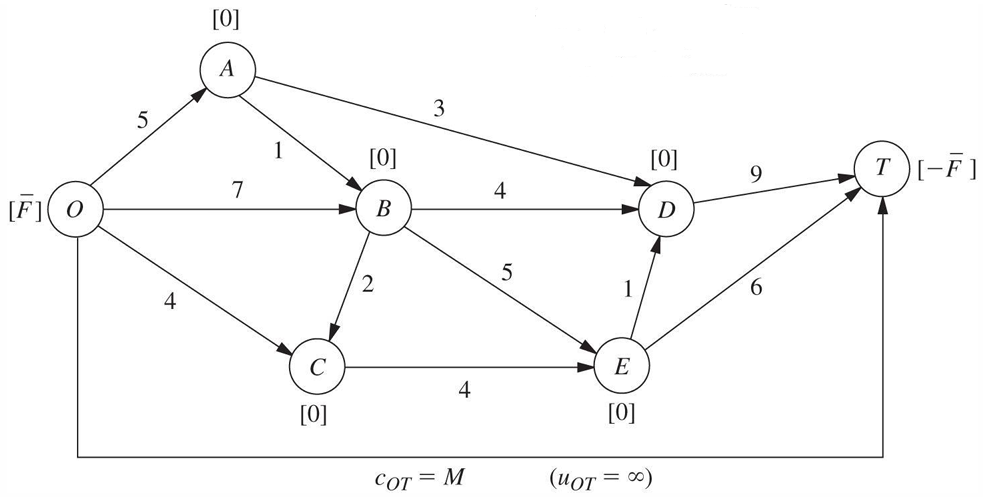
\includegraphics[scale=0.65]{images/flownetwork4.PNG}
\end{figure}

\noindent
For the maximum flow problem, we have a single supply node and a single demand node.
The supply and demand are set to $\bar{F}$, any upper bound on the maximum flow.
There are no costs on the arcs, but we add a single dummy arc with unlimited capacity straight from the supply node to the demand node.
This dummy arc has a high cost ($M$) to prevent it from being used.
Any flow not routed through the real network will be punished heavily, so the minimum-cost flow will attempt to minimize this, maximizing the real flow.

\subsection{The Network Simplex Method}
Just like other Simplex variants, the network Simplex method is an iterative algorithm.
At every iteration we check if the current BFS is optimal.
If not, we find the entering and leaving variables, and pivot to update the values of the basic variables.
If we have a minimum-cost flow problem with $n$ nodes, then the network Simplex method will always have $n - 1$ basic variables (also called \textbf{basic arcs}).
In this course we will not discuss how to construct an initial BFS, so just assume that we will always be given one.
Take a look at the following example:

\begin{figure}[h!]
    \centering
    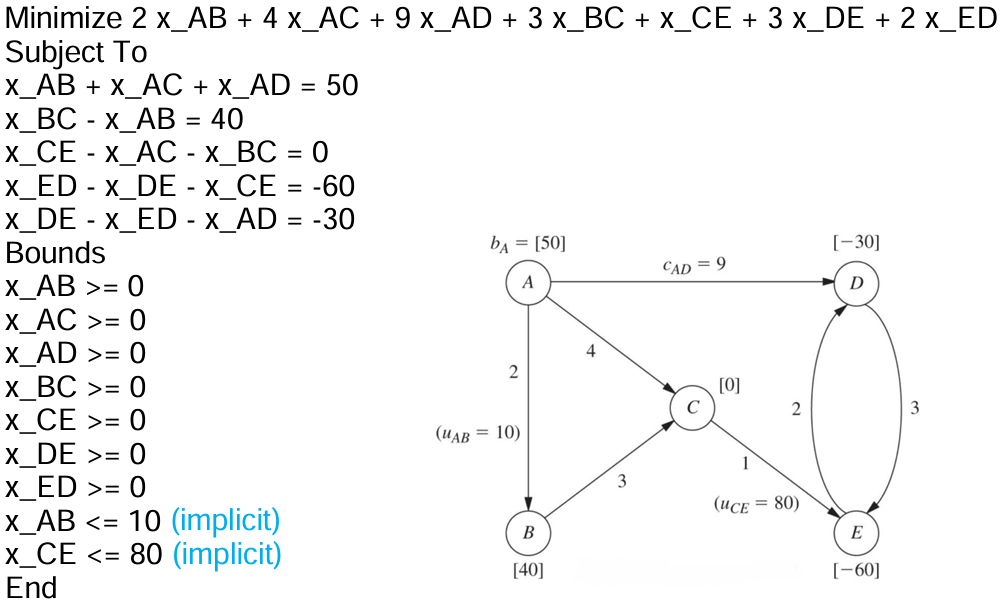
\includegraphics[scale=0.6]{images/networksimplex1.PNG}
\end{figure}

\newpage
\subsubsection{Upper Bound Technique}
Part of the reason why the network Simplex method is so efficient is because of the \textbf{upper bound technique}.
This technique allows us to implicitly encode arc capacity constraints, which means they do not count as functional constraints in the linear program.
The general idea is that we do not need a dedicated slack variable for the upper bound constraint $x_{ij} \leq u_{ij}$, because the slack is always equal to $u_{ij} - x_{ij}$.

\noindent
\\
When working with upper bounds, we need to watch out for the possibility of some basic variable hitting its upper bound whenever we increase the entering variable.
When this happens, we switch from working with $x_{ij}$ (the amount of flow above zero) to $u_{ij} - y_{ij}$, where $y_{ij}$ should be interpreted as the amount of flow below the upper bound.
At this point, $y_{ij}$ is nonbasic, and we can pivot to increase the entering variable.
If we substitute $u_{ij} - y_{ij}$ everywhere for $x_{ij}$, this causes the direction of the arc $i \rightarrow j$ to change:

\begin{figure}[h]
    \centering
    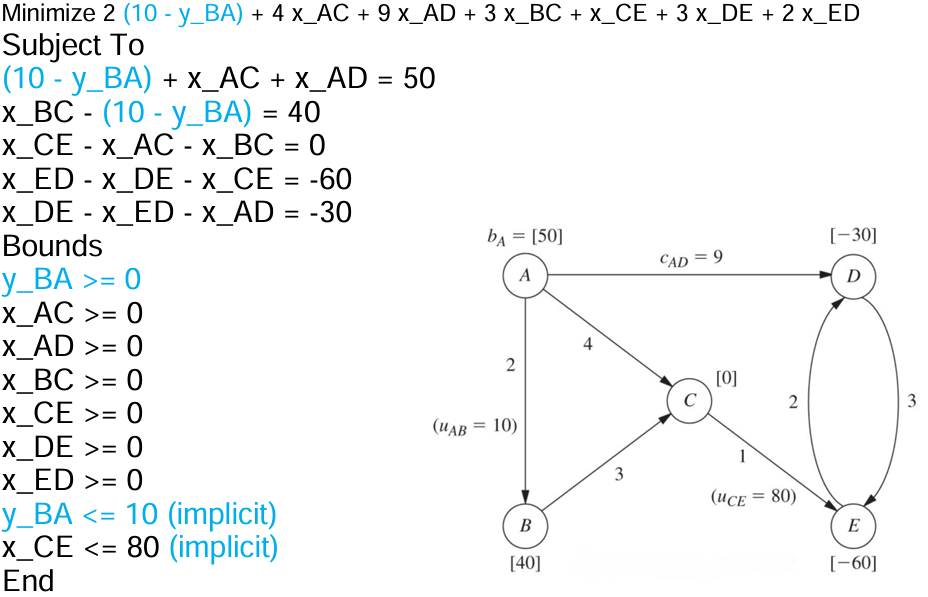
\includegraphics[scale=0.55]{images/networksimplex2.PNG}
    \\Substituting $u_{ij} - y_{ij}$ for $x_{ij}$ in the linear program.
\end{figure}

\begin{figure}[h]
    \centering
    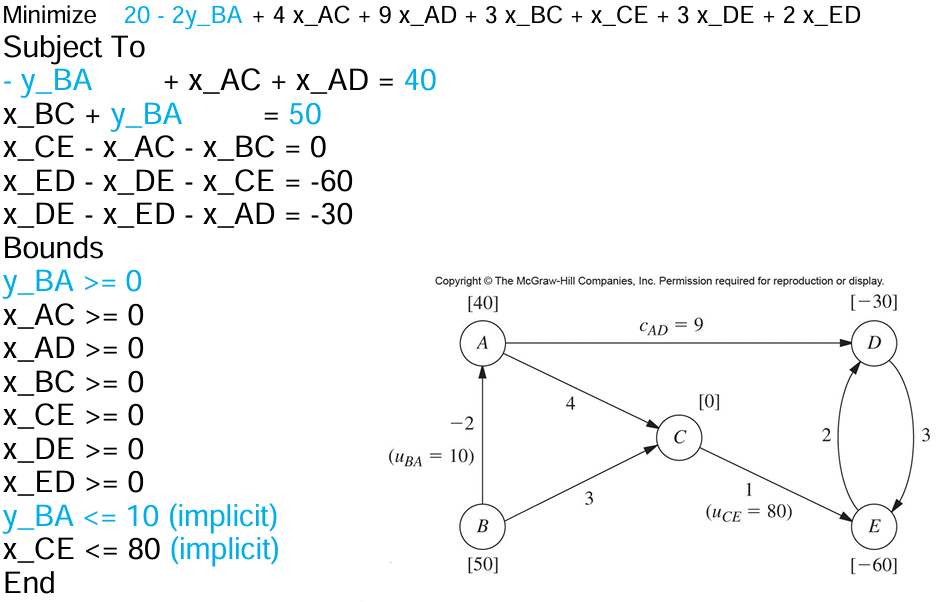
\includegraphics[scale=0.55]{images/networksimplex3.PNG}
    \\Arc $AB$ changes direction after substitution.
\end{figure}

\newpage
\noindent
Note how the supply and nodes $A$ and $B$ have also been adjusted, and that the cost of the arc is now negative.
The arc $AB$ has zero flow, but this actually means it is at maximum capacity in the original problem.

\subsubsection{Initial Arc Values}
When somebody gives you an initial BFS, you first need to compute the initial values of the basic arcs.
A solution will usually be given in the form of a \textbf{spanning tree}.
This is a tree with exactly $n - 1$ edges that connect all nodes in the network.
The idea is that the $n - 1$ edges in the spanning tree are the basic arcs, and the remaining arcs are nonbasic.
If the values of the basic arcs all obey the capacity and non-negativity constraints, then the spanning tree solution will be a \textbf{feasible spanning tree solution} (which is in one-to-one correspondence to a BFS).
Note that when pivoting, you deal with reversed arcs just the same as normal arcs.
Only at the end do you need to remember what the original direction of the arc was.
Assume that someone gives you the following initial spanning tree solution:

\begin{figure}[h]
    \centering
    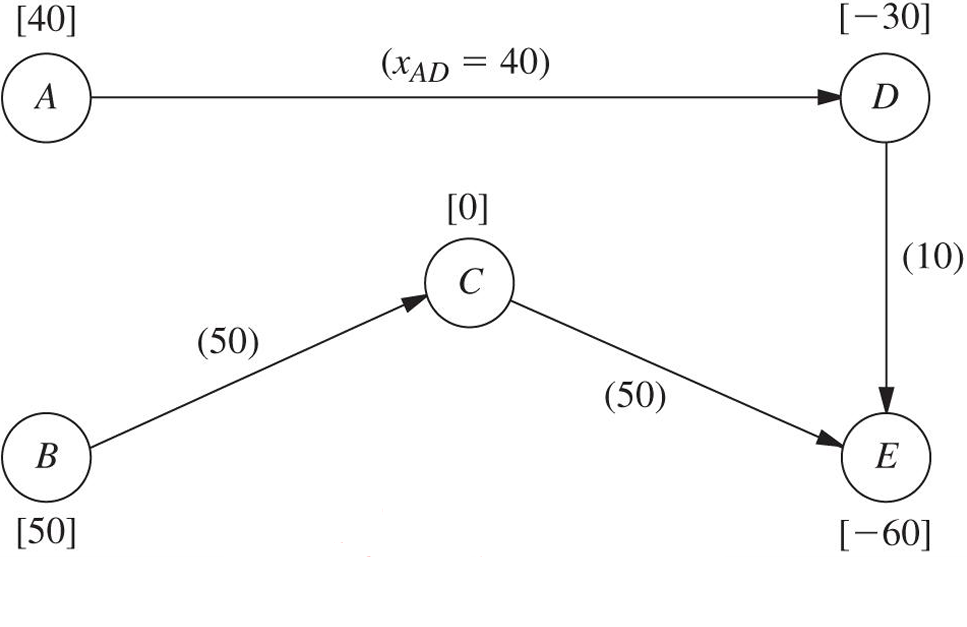
\includegraphics[scale=0.45]{images/networksimplex4.PNG}
\end{figure}

\noindent
Note that you are also told that the nonbasic arc $BA$ is the reverse of the original arc $AB$.
The values of the basic arcs can be calculated by solving the system of equations with the nonbasic arcs set to 0.
To compute the $Z$ value of the initial BFS, we sum the costs of the basic arcs multiplied by their flow values:
\[ Z = 40 \cdot 9 + 10 \cdot 3 + 50 \cdot 1 + 50 \cdot 3 + \mathbf{(10 \cdot 2)} \]

\noindent
The bold value is the cost of the reversed arc $BA$ (which is at maximum capacity).

\subsubsection{Pivoting}
To check whether the current BFS is optimal, we need to try if adding any nonbasic arc to the spanning tree will decrease the cost.
If we cannot find such an arc, then the current BFS is optimal.
Otherwise, we can use the most negative nonbasic arc as the entering variable.

\noindent
\\
The way we can check if a nonbasic arc can be added to the spanning tree is by going through all nonbasic arcs and adding them to the spanning tree with a value of $\theta$.
We then see how this increase of $\theta$ propagates through the network (similar to the closed loop technique in the transportation Simplex), and check if the cost increases or decreases as a result.
Here are all possible arcs that can be added to the spanning tree in our example:

\newpage
\begin{figure}[h]
    \centering
    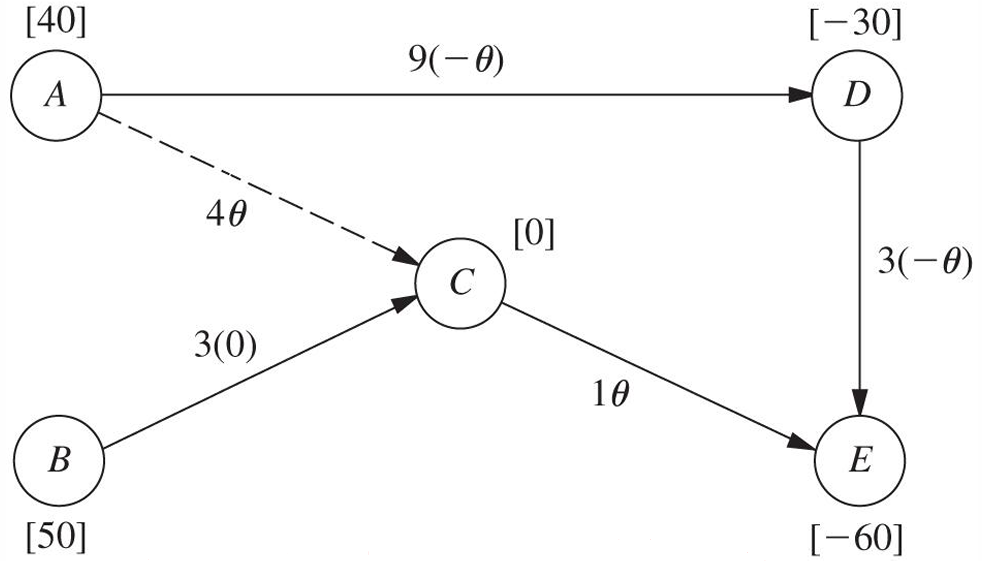
\includegraphics[scale=0.415]{images/networksimplex5.PNG}
    \\First option: $AC$. Reduced cost $= 1 - 3 - 9 + 4 = -7$ (per $\theta$).
\end{figure}

\begin{figure}[h]
    \centering
    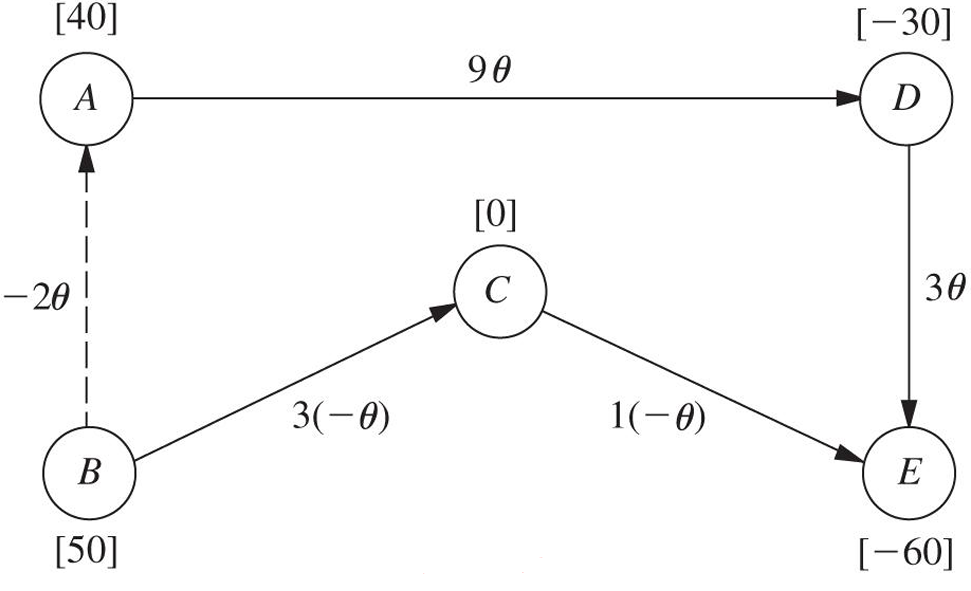
\includegraphics[scale=0.415]{images/networksimplex6.PNG}
    \\Second option: $BA$. Reduced cost $= -2 + 9 + 3 - 1 - 3 = 6$ (per $\theta$).
\end{figure}

\begin{figure}[h]
    \centering
    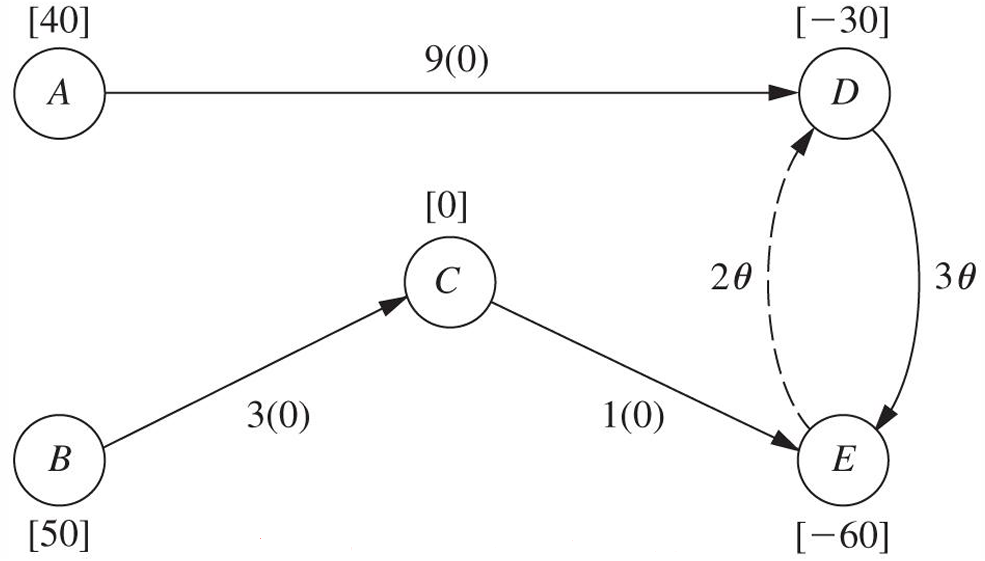
\includegraphics[scale=0.415]{images/networksimplex7.PNG}
    \\Third option: $ED$. Reduced cost $= 2 + 3 = 5$ (per $\theta$).
\end{figure}

\noindent
The first option is the most negative, so we will use arc $AC$ as the entering variable.
The next step is to identify the leaving basic variable and adjust the flow in the arcs.
The leaving variable will exit either because it hits zero or because it hits its upper bound (the entering variable might also hit its upper bound!).
If this happens make sure to reverse the arc directions and update the endpoints accordingly.
Our situation looks like this:

\newpage
\begin{figure}[h]
    \centering
    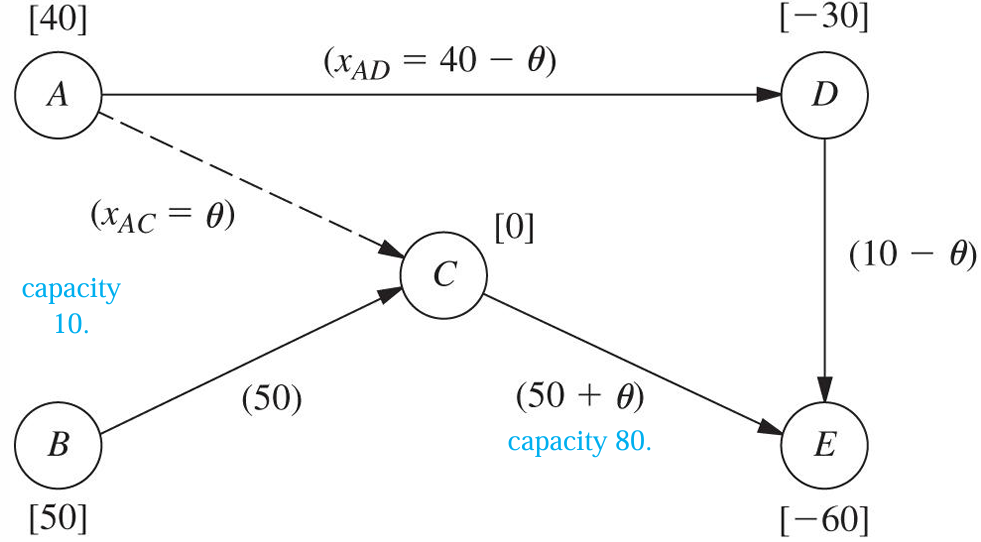
\includegraphics[scale=0.5]{images/networksimplex8.PNG}
\end{figure}

\noindent
When looking at the constraints within our $\theta$ loop, we can see that the $10 - \theta$ constraint is the most restrictive.
This means that we can set $\theta$ to 10 at most, and arc $DE$ will be the leaving variable:

\begin{figure}[h]
    \centering
    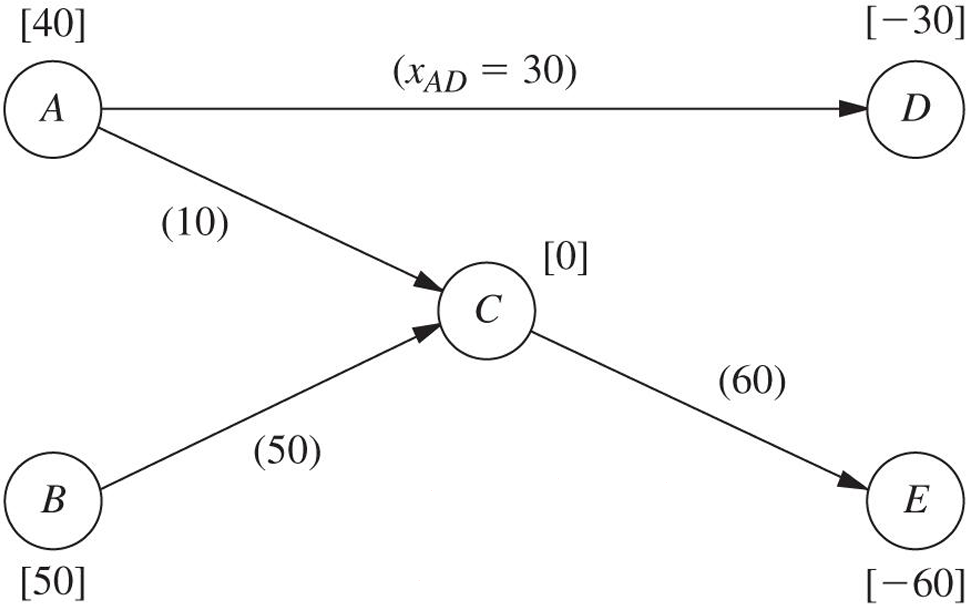
\includegraphics[scale=0.4]{images/networksimplex9.PNG}
\end{figure}

\noindent
We have now completed one iteration of the network Simplex method.
The rest of the pivots are as follows:

\begin{figure}[h!]
    \centering
    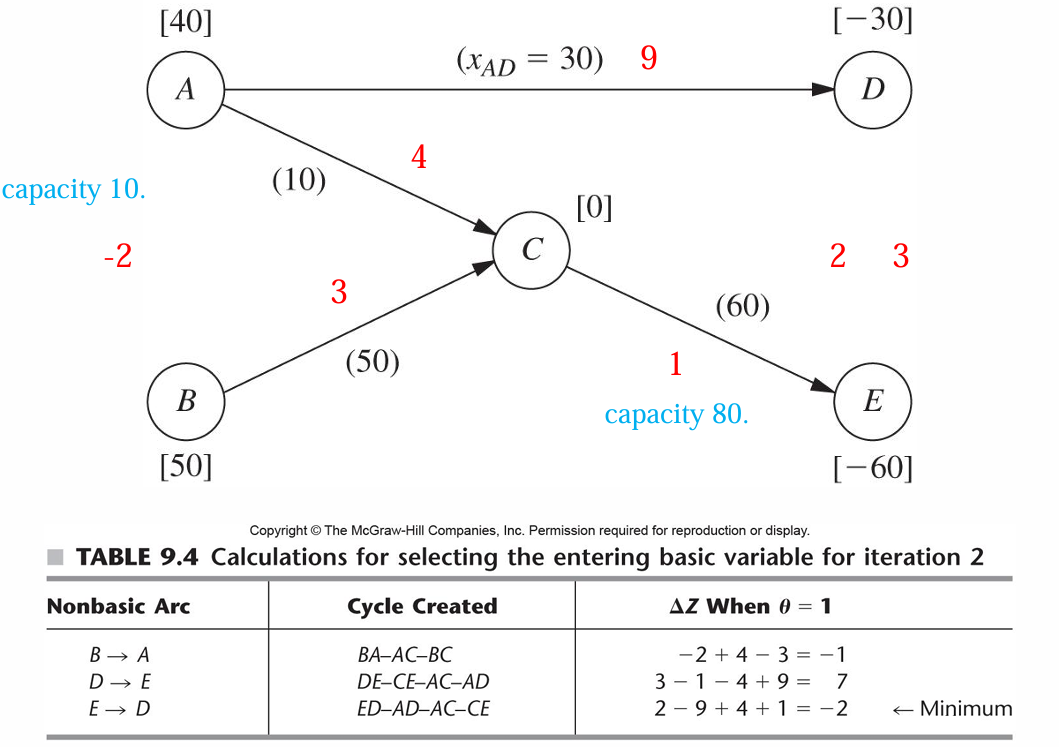
\includegraphics[scale=0.55]{images/networksimplex10.PNG}
\end{figure}

\newpage
\begin{figure}[h!]
    \centering
    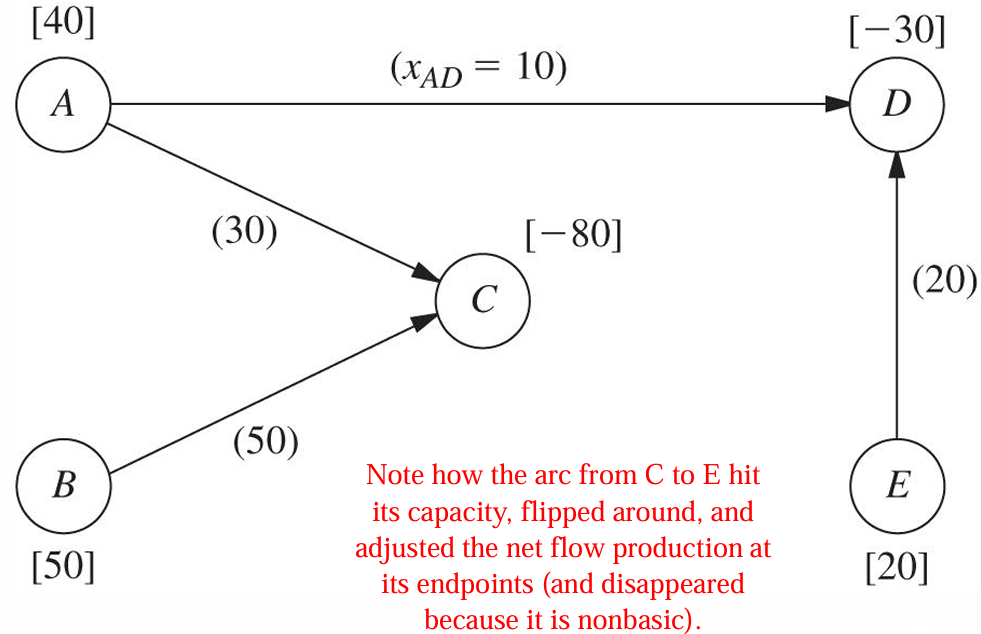
\includegraphics[scale=0.45]{images/networksimplex11.PNG}
\end{figure}

\begin{figure}[h!]
    \centering
    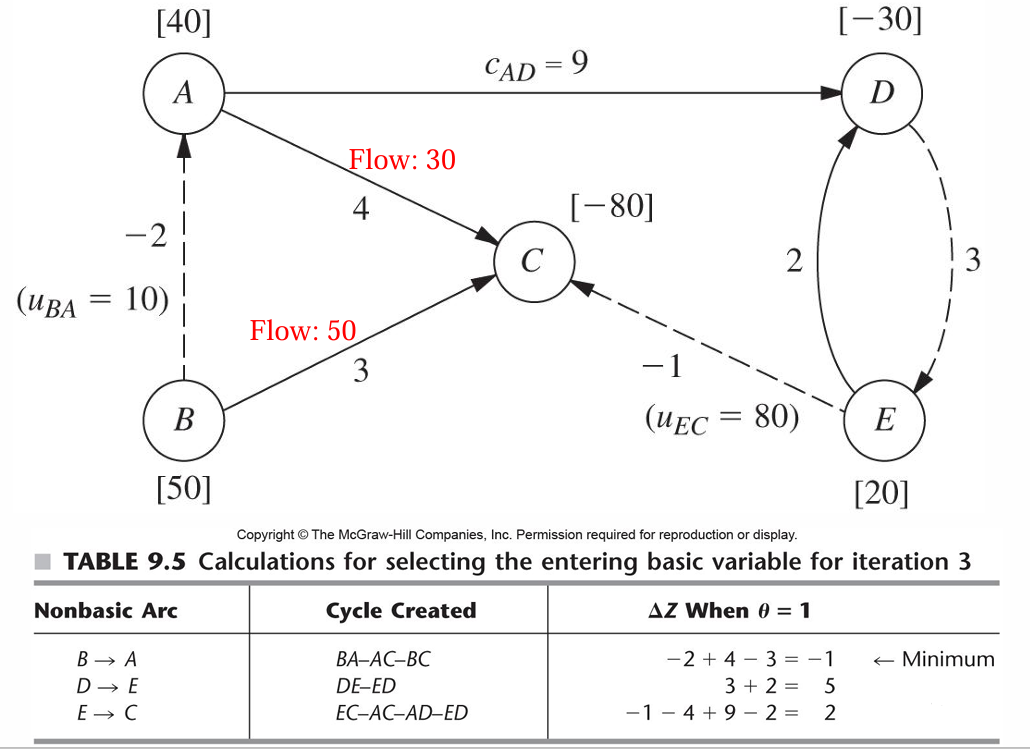
\includegraphics[scale=0.55]{images/networksimplex12.PNG}
\end{figure}

\begin{figure}[h!]
    \centering
    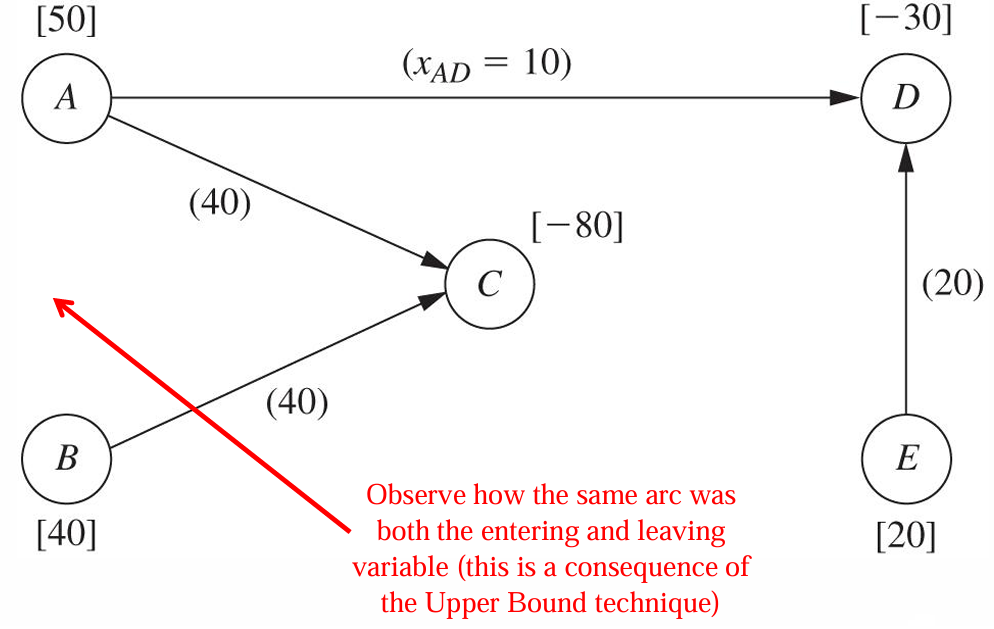
\includegraphics[scale=0.45]{images/networksimplex13.PNG}
\end{figure}

\newpage
\begin{figure}[h]
    \centering
    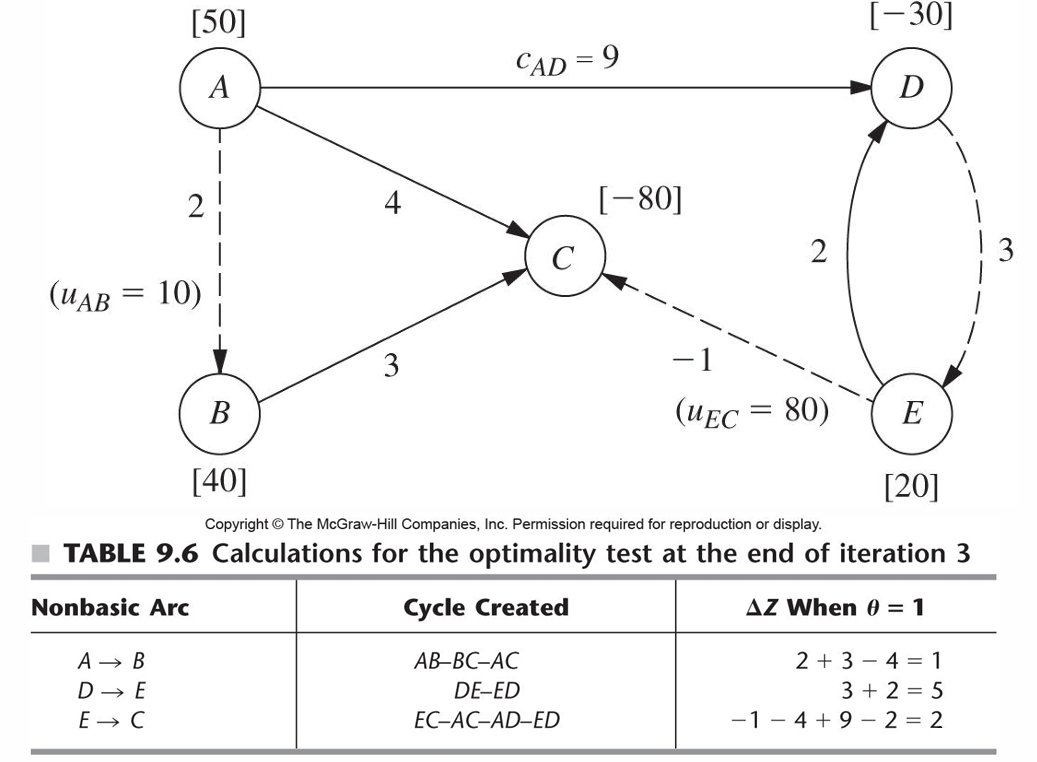
\includegraphics[scale=0.55]{images/networksimplex14.PNG}
\end{figure}

\noindent
The final BFS is optimal, as there are no more negative reduced costs.
To get the final solution, we need to flip back any arcs that are still pointing the wrong way.
In this example, the only arc to fix is the reverse arc from $E$ to $C$:

\begin{figure}[h]
    \centering
    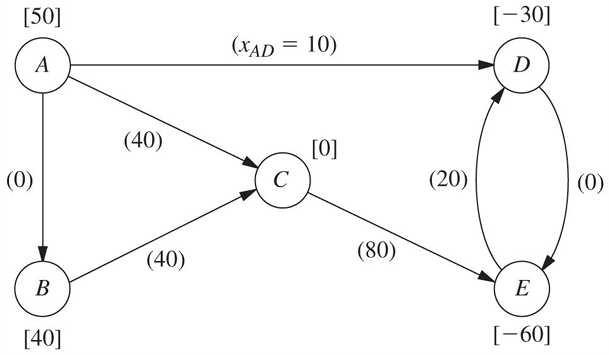
\includegraphics[scale=0.8]{images/networksimplex15.PNG}
\end{figure}

%
% Topic 7 - Integer Programming
%
\newpage
\section{Integer Programming}
There are (at least) two factors limiting what we can do with computers.
The first is that some problems are just inherently hard to solve (NP-hard).
The second is the difficulty of explaining to a computer what we want it to do.
\textbf{Integer programming} can be seen as a (partial) solution to both these problems.
Integer programming can, unlike linear programming, often be used to solve NP-hard problems, and we can use it to simply tell a computer \textit{what} we want it to do, instead of \textit{how}.

\subsection{Modelling Integer Programming Problems}
The key difference between linear programming and integer programming is that in integer programming we can restrict some variables to be integers.
This is also called \textbf{mixed-integer linear programming}, but it is essentially the same thing.
An important subcategory of integer programming is \textbf{binary integer programming (BIP)}.
This is where all the integer variables in the program are binary (i.e. either 0 or 1).
In operations research, binary variables are often used to model decisions, such as whether to build a factory or not.
Take the following example:

\begin{figure}[h]
    \centering
    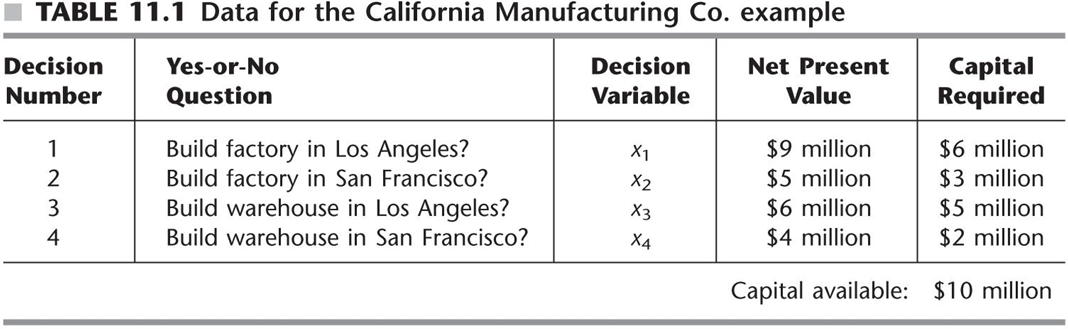
\includegraphics[scale=0.7]{images/integerprogramming1.PNG}
\end{figure}

\noindent
We want to know if it is worth it to open a new factory, and if so, where to build it.
We are also allowed to open at most one warehouse, but only in a city where we have a factory.
How should we spend our \$10 million budget to maximize profit?
We can model this problem as the following integer program:
\begin{align*}
    &\mathrm{max} \quad Z = 9x_1 + 5x_2 + 6x_3 + 4x_4 \\[2pt]
    &\mathrm{s.t.} \quad 
    \begin{array}[t]{r c l}
        6x_1 + 3x_2 + 5x_3 + 2x_4 & \leq & 10 \\
        x_3 + x_4 & \leq & 1 \\
        -x_1 + x_3 & \leq & 0 \\
        -x_2 + x_4 & \leq & 0
     \end{array}
\end{align*}

\noindent
Where $x_1, x_2, x_3, x_4$ are binary variables.

\subsubsection{Auxiliary Binary Variables}
To help some problems be modelled as integer programs, we can introduce \textbf{auxiliary binary variables}.
These variables are introduced solely to help formulate the problem, instead of being part of the decision variables.
Auxiliary binary variables can be used to model many novel cases in integer programming, such as the following examples:

\newpage
\noindent
\textbf{Either-Or Constraints:}
Consider the case where a choice must be made between two constraints, so that only one must hold (the other one can hold as well, but is not required to).
Take the following example:
\begin{align*}
    \begin{array}[t]{r c l}
        3x_1 + 2x_2 & \leq & 18 \\
        x_1 + 4x_2 & \leq & 16
     \end{array}
\end{align*}

\noindent
At least one of these inequalities must hold, but not necessarily both.
This requirement must be reformulated to fit into the linear programming format where all constraints must hold.
We can solve this by introducing an auxiliary binary variable $y$:
\begin{align*}
    \begin{array}[t]{r c l}
        3x_1 + 2x_2 & \leq & 18 + My \\
        x_1 + 4x_2 & \leq & 16 + M(y - 1)
     \end{array}
\end{align*}

\noindent
\textbf{K out of N Constraints:}
Whereas the previous example required only one of two constraints to hold, here we present the more general case where at least $K$ out of $N$ constraints must hold.
This is a pretty straightforward extension of the previous example, and can be solved by introducing $N$ auxiliary binary variables $y_1, y_2, ..., y_N$:
\begin{align*}
    \begin{array}[t]{r c l}
        ... & \leq & d_1 + My_1 \\
        ... & \leq & d_2 + My_2 \\
        & \vdots & \\
        ... & \leq & d_N + My_N \\
        \sum_i y_i & = & N - K
     \end{array}
\end{align*}

\noindent
\textbf{Functions with N Possible Values:}
Consider the situation where a given function is required to take on any one of $N$ given values:
\[ f(x_1, x_2, ... , x_n) = \{ d_1, d_2, ... d_N \} \]

\noindent
This can once again be modelled by introducing $N$ auxiliary binary variables $y_1, y_2, ... , y_N$:
\begin{align*}
    \begin{array}[t]{r c l}
        f(x_1, x_2, ... , x_n) & = & d_1y_1 + d_2y_2 + ... + d_Ny_N \\
        y_1 + y_2 + ... + y_N & = & 1
     \end{array}
\end{align*}

\noindent
\textbf{Fixed-Cost Problem:}
Consider the case where $x_i$ is the amount of product $i$ to produce, and $c_i$ is the cost of producing one unit of product $i$.
If $x_i = 0$, i.e. we don't produce any of product $i$, then we do not build a factory for product $i$.
If $x_i > 0$, then we do have to build factory at a fixed cost $F_i$.
We want to minimize the total cost of production:
\begin{equation*}
    \begin{cases}
        c_ix_i + F_i & \text{if } x_i > 0\\
        0 & \text{if } x_i = 0
    \end{cases}       
\end{equation*}

\noindent
If we are dealing with a minimization problem, can model this as an integer program by introducing an auxiliary binary variable $y_i$ for every $x_i$:
\begin{align*}
    &\mathrm{min} \quad Z = ... + c_ix_i + ... + F_iy_i \\[2pt]
    &\mathrm{s.t.} \quad 
    \begin{array}[t]{r c l}
        & \vdots & \\
        x_i & \leq & My_i \\
        & \vdots &
     \end{array}
\end{align*}

\newpage
\noindent
\textbf{Binary Representation of General Integer Variables:}
Suppose we have a general integer programming problem where most variables are binary, but the presence of a few general integer variables stops the problem from being solved by a fast BIP-solver.
A nice way to circumvent this is to use the binary representation of each general integer variable.
For example, suppose we have an integer programming problem with just two general integer variables:
\begin{align*}
    \begin{array}[t]{r c l}
        x_1 & \leq & 5 \\
        2x_1 + 3x_2 & \leq & 30
     \end{array}
\end{align*}

\noindent
Where both $x_1$ and $x_2$ also have non-negativity constraints.
If the bounds of an integer variable are of the following form:
\[ 0 \leq x_i \leq u_i \]

\noindent
Then the binary representation of $x_i$ is:
\[ x_i = \sum_{j = 0}^N 2^jy_j, \text{ where } 2^N \leq u_i < 2^{N + 1} \]

\noindent
Where $y_j$ are auxiliary binary variables.
If we substitute this binary representation into the original problem, we can solve the problem as a BIP problem:
\begin{align*}
    \begin{array}[t]{r c l}
        y_0 + 2y_1 + 4y_2 & \leq & 5 \\
        2y_0 + 4y_1 + 8y_2 + 3y_3 + 6y_4 + 12y_5 + 24y_6 & \leq & 30
     \end{array}
\end{align*}

\noindent
\textbf{Maximizing Variables:}
Suppose we have normal (non-integral) variables $x_1, x_2$ and $z$.
Using an auxiliary binary variable $y$, we can model the relation $z = \max(x_1, x_2)$ as follows:
\begin{align*}
    \begin{array}[t]{r c l}
        z & \geq & x_1 \\
        z & \geq & x_2 \\
        z & \leq & x_1 + My \\
        z & \leq & x_2 + M(y - 1)
     \end{array}
\end{align*}

\noindent
\textbf{AND Operator:}
Suppose we have binary variables $x_1, x_2$ and $z$.
We can model the relation $z = x_1 \land x_2$ as follows:
\begin{align*}
    \begin{array}[t]{r c l}
        z & \leq & x_1 \\
        z & \leq & x_2 \\
        z & \geq & x_1 + x_2 - 1
     \end{array}
\end{align*}

\subsubsection{Complex Examples}
\textbf{Example 1 - Making Choices with Continuous Decision Variables:}
A company has created three new products, but only wants to expand their stock with two of them.
Each of these products can be produced in either of two plants, but for administrative reasons one plant must become the sole producer of both products.
There is a limited amount of time available for production in each plant, and each product also has a maximum sales capacity (see the table below).
The company wants to maximize profit.
Note that the production volumes do not have to be integral.

\newpage
\begin{figure}[h]
    \centering
    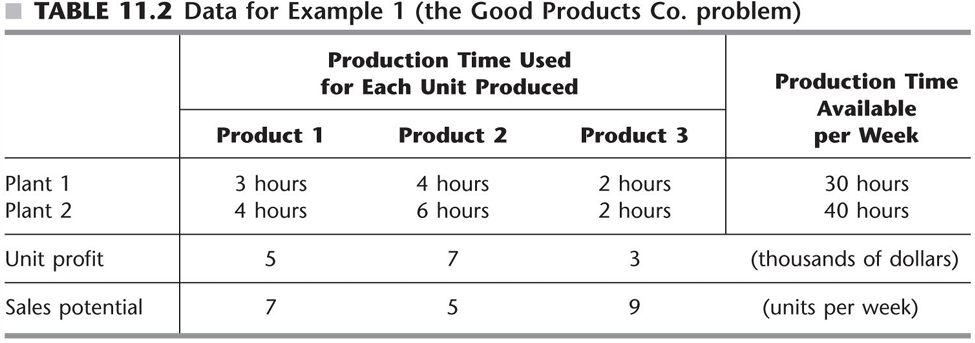
\includegraphics[scale=0.7]{images/integerprogramming2.PNG}
\end{figure}

\noindent
We can model this problem as the following integer program:
\begin{align*}
    &\mathrm{max} \quad Z = 5x_1 + 7x_2 + 3x_3 \\[2pt]
    &\mathrm{s.t.} \quad 
    \begin{array}[t]{r c l}
        x_1 & \leq & 7 \\
        x_2 & \leq & 5 \\
        x_3 & \leq & 9 \\
        x_1 & \leq & My_1 \\
        x_2 & \leq & My_2 \\
        x_3 & \leq & My_3 \\
        y_1 + y_2 + y_3 & \leq & 2 \\
        3x_1 + 4x_2 + 2x_3 - My_4 & \leq & 30 \\
        4x_1 + 6x_2 + 2x_3 + My_4 & \leq & 40 + M
     \end{array}
\end{align*}

\noindent
Where $x_1, x_2, x_3$ are continuous variables with non-negativity constraints, and $y_1, y_2, y_3, y_4$ are binary variables.

\noindent
\\
\textbf{Example 2 - Violating Proportionality:}
A company with a lineup of three products wants to buy TV ads.
The company wants to buy 5 ads in total, and will distribute them among the three products.
Each product can have at most 3 ads, so each product will have 0-3 ads allocated to it.
The company wants to maximize profit, given the following table:

\begin{figure}[h]
    \centering
    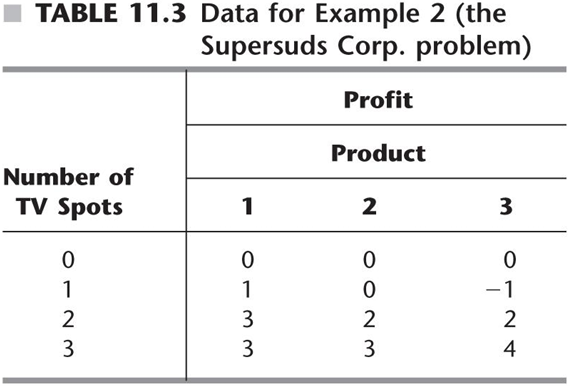
\includegraphics[scale=0.7]{images/integerprogramming3.PNG}
\end{figure}

\noindent
This is a tricky problem since the profit does not grow proportionally with the number of ads.
We can model this problem as the following integer program:

\newpage
\begin{align*}
    &\mathrm{max} \quad Z = y_{11} + 3y_{12} + 3y_{13} + 2y_{22} + 3y_{23} - y_{31} + 2y_{32} + 4y_{33} \\[2pt]
    &\mathrm{s.t.} \quad 
    \begin{array}[t]{r c l}
        y_{11} + y_{12} + y_{13} & \leq & 1 \\
        y_{21} + y_{22} + y_{23} & \leq & 1 \\
        y_{31} + y_{32} + y_{33} & \leq & 1 \\
        y_{11} + 2y_{12} + 3y_{13} + y_{21} + 2y_{22} + 3y_{23} + y_{31} + 2y_{32} + 3y_{33} & = & 5
     \end{array}
\end{align*}

\noindent
Where $y_{ij}$ are all binary variables.

\noindent
\\
\textbf{Example 3 - Covering all Characteristics:}
An airline company has to assign its three crews to cover all 11 flights.
The possible flight sequences and corresponding costs are given in the following table:

\begin{figure}[h]
    \centering
    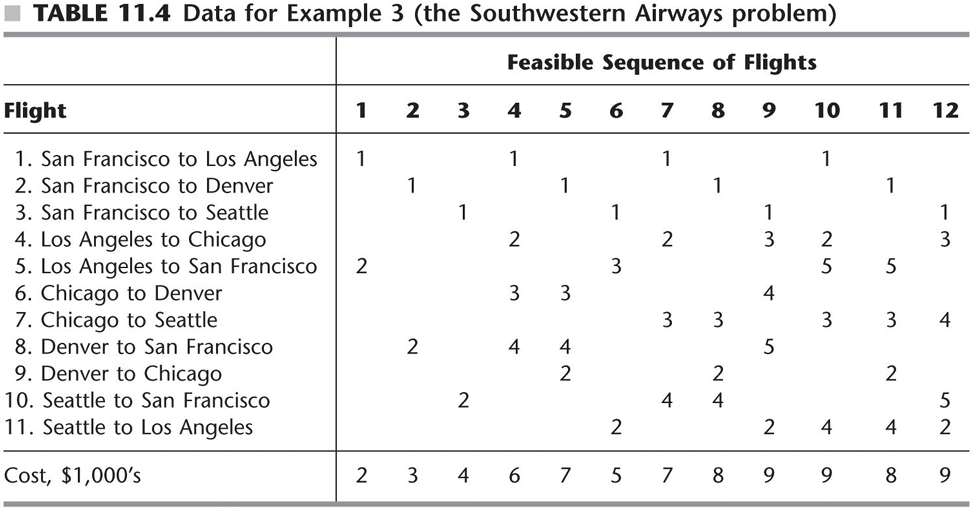
\includegraphics[scale=0.7]{images/integerprogramming4.PNG}
\end{figure}

\noindent
The company needs to choose three columns such that every row is covered at least once (i.e. a set covering problem).
The goal is to minimize the total cost.
We can model this problem as the following integer program:

\begin{align*}
    &\mathrm{min} \quad Z = 2x_1 + 3x_2 + 4x_3 + 6x_4 + 7x_5 + 5x_6 + 7x_7 + 8x_8 + 9x_9 + 9x_{10} + 8x_{11} + 9x_{12} \\[2pt]
    &\mathrm{s.t.} \quad 
    \begin{array}[t]{r c l}
        x_1 + x_4 + x_7 + x_{10} & \geq & 1 \\
        x_2 + x_5 + x_8 + x_{11} & \geq & 1 \\
        x_3 + x_6 + x_9 + x_{12} & \geq & 1 \\
        x_4 + x_7 + x_9 + x_{10} + x_{12} & \geq & 1 \\
        x_1 + x_6 + x_{10} + x_{11} & \geq & 1 \\
        x_4 + x_5 + x_9 & \geq & 1 \\
        x_7 + x_8 + x_{10} + x_{11} + x_{12} & \geq & 1 \\
        x_2 + x_4 + x_5 + x_9 & \geq & 1 \\
        x_5 + x_8 + x_{11} & \geq & 1 \\
        x_3 + x_7 + x_8 + x_{12} & \geq & 1 \\
        x_6 + x_9 + x_{10} + x_{11} + x_{12} & \geq & 1 \\
        \sum_i x_i & = & 3
     \end{array}
\end{align*}

\noindent
Where $x_i$ are all binary variables.

\newpage
\subsection{Solving Integer Programs}
In a formal sense, solving an integer program is NP-hard.
However, a linear program can be solved very easily.
One natural idea is to \textit{relax} the integrality constraints to obtain a linear program, for example by replacing "$x$ is binary" with "$0 \leq x \leq 1$".
This is called the \textbf{LP-relaxation} of the integer program.
Solving the LP-relaxation can help us solve the integer program, but the solution will not necessarily be feasible nor optimal:

\begin{figure}[h]
    \centering
    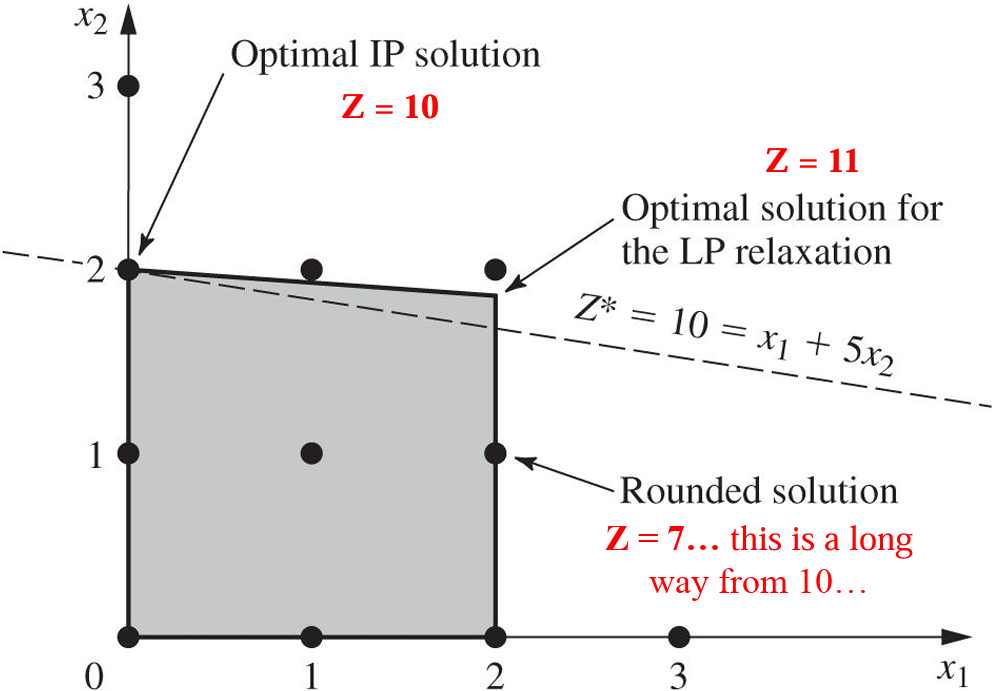
\includegraphics[scale=0.5]{images/ipsolving1.PNG}
\end{figure}

\noindent
Simply solving the LP-relaxation and rounding the solution is problematic, but it does tell us something about the solution of the integer program.
For maximization problems, the optimal value of the LP-relaxation is always an \textbf{upper bound} on the optimal value of the integer program.
For minimization problems, the optimal value of the LP-relaxation is always a \textbf{lower bound} on the optimal value of the integer program.

\subsubsection{Branch-and-Bound}
One straight forward way of solving an integer program is to simply enumerate all possible values for the integer / binary variables, and solve the corresponding linear programs.
Of course, there are far too many values to check, but in practice many of these possible values can be excluded because they cannot possibly improve the current best solution.
We can use LP-relaxations to give us a quickly computable bound, which we can use to say "don't bother going down this search path, because even with relaxed variables we can't improve upon the current best solution".
This is called the \textbf{branch-and-bound} method:

\begin{itemize}
    \item \textbf{Branching:} guessing a value for a binary variable.
    \item \textbf{Bounding:} using relaxations to get a bound on the optimal value.
\end{itemize}

\noindent
The first step of the branch-and-bound method is to solve the LP-relaxation of the integer program.
In this maximization example with binary variables $x_1, x_2, x_3$ and $x_4$, we find an optimal solution $(\frac{5}{6}, 1, 0, 1)$ with $Z = 16$.
This means that we can use $Z = 16$ as an upper bound on the optimal value of the integer program.
Since the solution is not integral, we need to branch on one of the variables.
We choose to branch on $x_1$, and solve the corresponding linear programs:

\newpage
\begin{figure}[h]
    \centering
    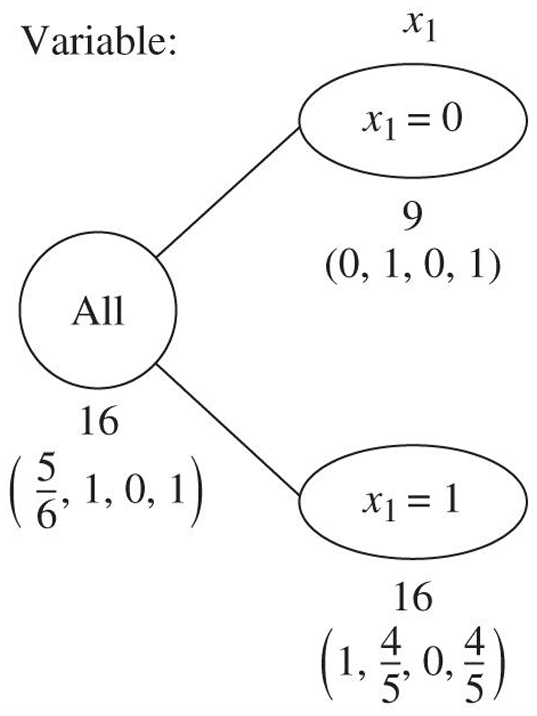
\includegraphics[scale=0.35]{images/ipsolving2.PNG}
\end{figure}

\noindent
Note that the branch with $x_1 = 0$ produces an integral solution with $Z = 9$.
Since this is an integral solution, it must be the optimal solution to this branch.
This means that we can store this solution as the \textbf{incumbent} (the best feasible solution found so far), with its value denoted by $Z^* = 9$:

\begin{figure}[h]
    \centering
    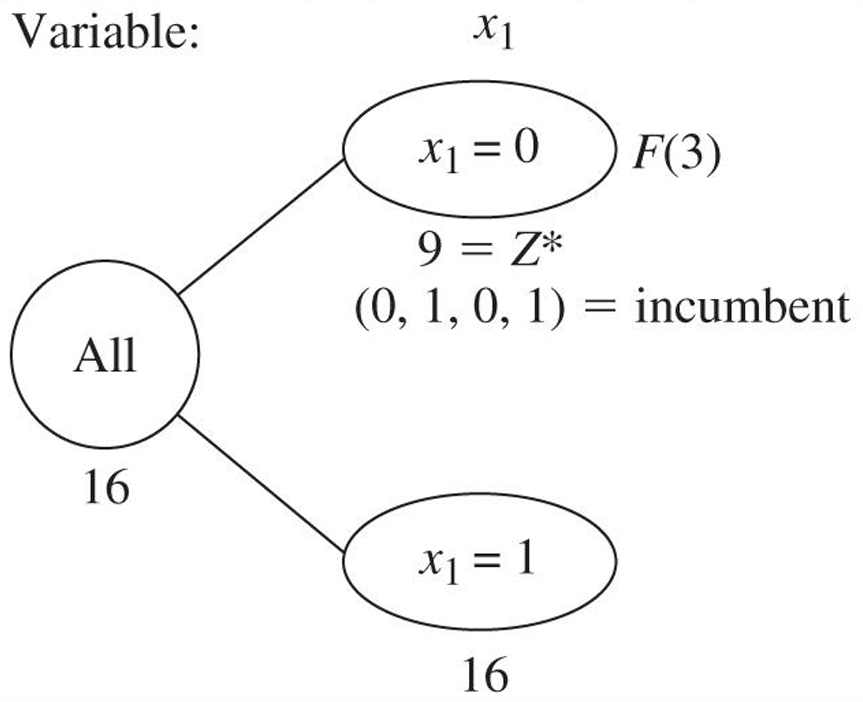
\includegraphics[scale=0.325]{images/ipsolving3.PNG}
\end{figure}

\noindent
Since this branch has been solved, we can \textbf{fathom} (dismiss) this branch, and move on to the next branch.
This is denoted by the $F(3)$ after the branch, showing by which rule it was fathomed:

\begin{enumerate}
    \item Its bound is $\leq Z^*$.
    \item Its LP-relaxation has no feasible solutions.
    \item The solution to its LP-relaxation is integral (if it is $> Z^*$, it becomes the new incumbent).
\end{enumerate}

\begin{figure}[h!]
    \centering
    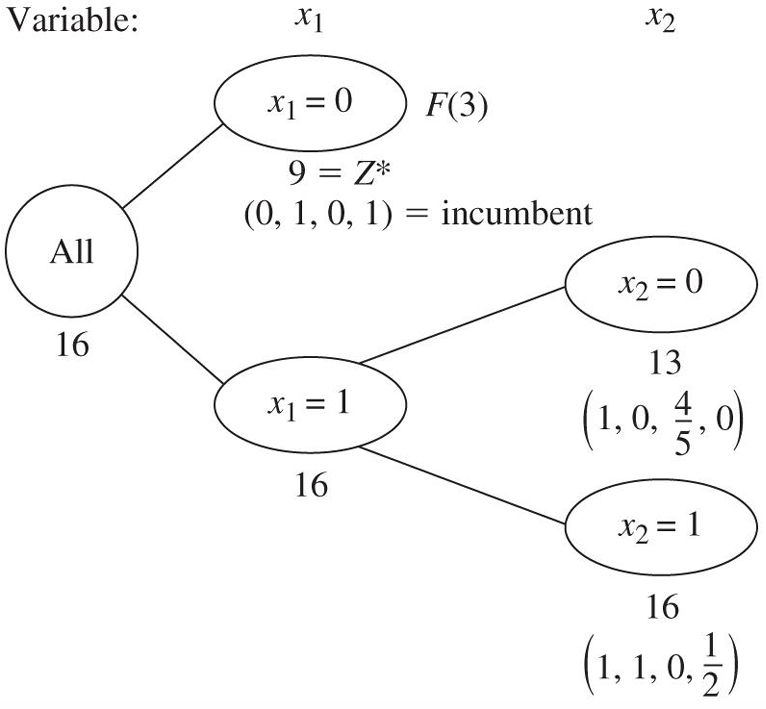
\includegraphics[scale=0.425]{images/ipsolving4.PNG}
\end{figure}

\newpage
\noindent
Branching on the $x_1 = 1$ branch, we find two new branches with $x_2 = 0$ and $x_2 = 1$.
Both of these branches cannot be fathomed, as neither pass any of the rules shown earlier.
Whenever there are multiple branches to choose from, you should first choose the one created most recently, then break ties by choosing the one with the largest upper bound.
This means that we will continue branching on $x_2 = 1$:

\begin{figure}[h]
    \centering
    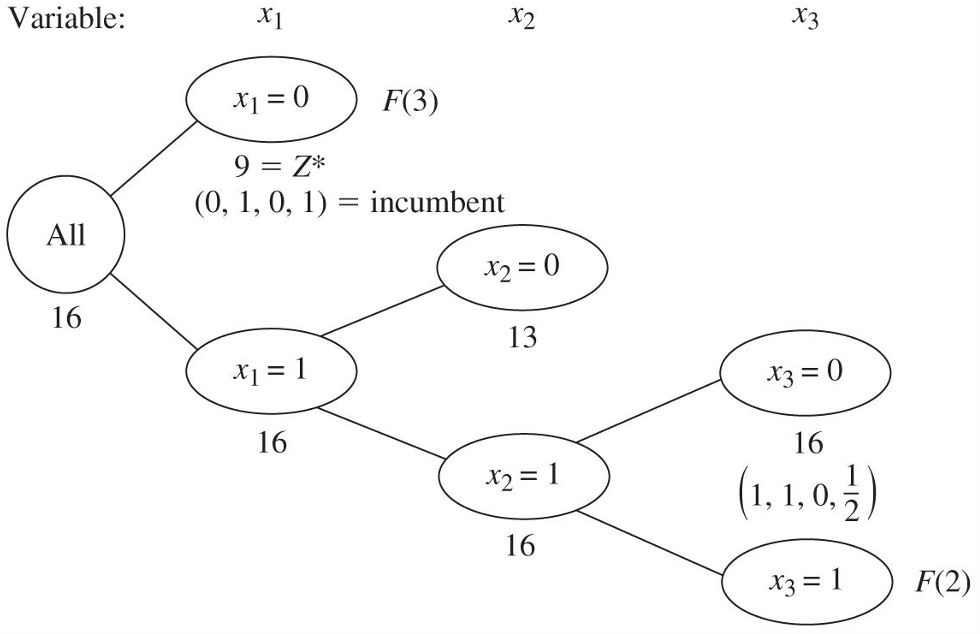
\includegraphics[scale=0.5]{images/ipsolving5.PNG}
\end{figure}

\noindent
The branch with $x_3 = 1$ is fathomed, as it has no feasible solutions.
We continue branching on $x_3 = 0$:

\begin{figure}[h]
    \centering
    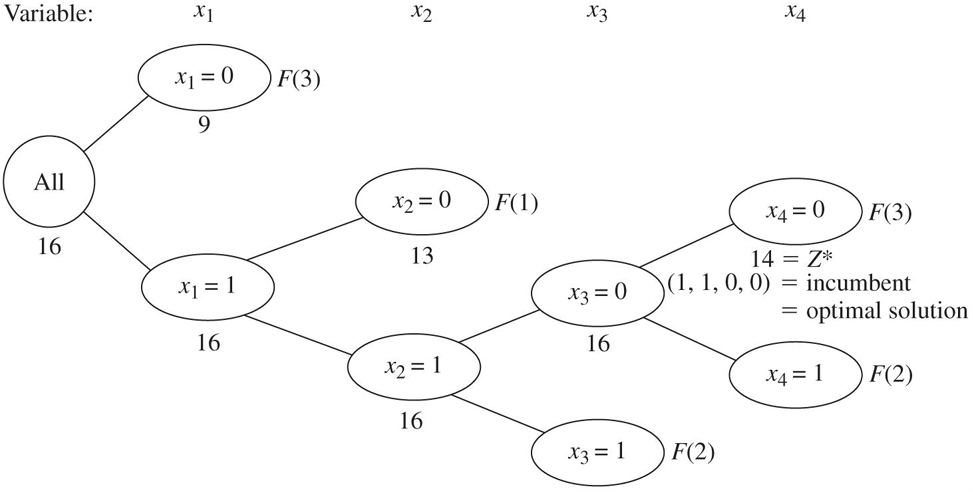
\includegraphics[scale=0.6]{images/ipsolving6.PNG}
\end{figure}

\noindent
The branch with $x_4 = 1$ is fathomed, as it has no feasible solutions.
The branch with $x_4 = 0$ produces an integral solution with $Z = 14$.
Since this is a higher value than the incumbent, we update the incumbent to $Z^* = 14$.
After we update the incumbent, we apply the fathoming rules again, and find that the branch with $x_2 = 0$ that was still open can now be fathomed, as its bound is less than $Z^*$.
Since all branches are now closed, we have found the optimal solution to the integer program.

\noindent
\\
Note that, just because a binary variable is equal to 0 or 1 in the LP-relaxation of a branch, does not mean that we can avoid branching on it.
If in the first branching the value of $x_2$ would have been 0 or 1 in both cases, then we would still have to branch on it.
This is because constraints added later might destroy its integrality.

\noindent
\\
In this example, we just branched on the variables in order.
This is completely fine, but in practice there are better ways of choosing which variable to branch on.

\newpage
\subsubsection{Branch-and-Bound for Mixed Integer Programs}
The above example showed how to solve a binary integer program using branch-and-bound.
The procedure for general integer programs (where there are integer variables) is very similar.
Suppose we have a non-negative integer variable $x$ that has a value of 7.4 in the LP-relaxation.
We can branch on this variable by creating two branches, one where $x \leq 7$ and one where $x \geq 8$.
Note that because we are now branching with ranges, we might have to branch on the same variable more than once.

\subsubsection{Branch-and-Cut}
Even though branch-and-bound is a powerful method, it can still be very slow for large problems.
\textbf{Branch-and-cut} is a method that combines branch-and-bound with techniques to strengthen the LP-relaxation.
The idea is to "cut off" large pieces of the feasible region of the LP-relaxations, without cutting off any feasible integer solutions.
The four most common techniques are the following:

\noindent
\\
\textbf{Fixing Variables:}
If one value of a variable cannot satisfy a certain constraint, even when the other variables equal their best values for trying to satisfy the constraint, then that variable should be fixed at its other value.
For example:
\[ 5x_1 + x_2 - 2x_3 \leq 2 \quad \Rightarrow \quad x_1 = 0, \quad \text{since} \quad 5(1) + 1(0) - 2(1) > 2 \]

\noindent
\textbf{Eliminating Redundant Constraints:}
If a functional constraint satisfies even the most challenging binary solution, then it has been made redundant by the binary constraints and can be eliminated from further consideration.
For example:
\[ 3x_1 + 2x_2 \leq 6 \quad \text{is redundant, since} \quad 3(1) + 2(1) \leq 6 \]

\noindent
\textbf{Tightening Constraints:}
\begin{figure}[h]
    \centering
    \begin{minipage}{.5\textwidth}
      \centering
      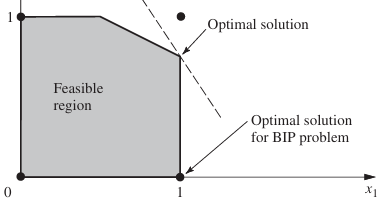
\includegraphics[scale=0.75]{images/ipsolving7.PNG}
      \\Original LP-relaxation.
    \end{minipage}%
    \begin{minipage}{.5\textwidth}
      \centering
      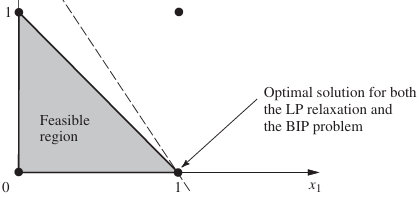
\includegraphics[scale=0.75]{images/ipsolving8.PNG}
      \\LP-relaxation with tightened constraints.
    \end{minipage}
\end{figure}

\noindent
\textbf{Cutting Planes:}
Cutting planes are constraints that we add to cut off parts of the feasible region of the LP-relaxation.
For example:
\[ 6x_1 + 3x_2 + 5x_3 + 2x_4 \leq 10 \quad \text{implies} \quad x_1 + x_2 + x_4 \leq 2 \]

\noindent
Note that this does not replace the original constraint, but it adds to it.

%
% Topic 8 - Nonlinear Programming
%
\newpage
\section{Nonlinear Programming}
Just like linear programming, the goal of \textbf{nonlinear programming (NLP)} is to optimize a function subject to a set of constraints.
A program is nonlinear if its objective function or any of its constraints are nonlinear.
There is no single algorithm that can solve all nonlinear programs, but there are many methods that can be used to solve different types of nonlinear programs.
Without any special structure, nonlinear programs cannot be solved to optimality.
However, the more structure a program has, the more efficiently we can handle it.
The most important distinction in nonlinear programming is between \textbf{convex} and \textbf{non-convex} programs.

\subsection{Convexity}
A \textbf{convex program} is any nonlinear program where you maximize a concave function or minimize a convex function, both over a \textbf{convex feasible region}.

\subsubsection{Convex Functions}
For one-variable functions, a function is convex if the line segment between any two points on the graph of the function lies above the graph.
Similarly, a function is concave if the line segment lies below the graph:

\begin{figure}[h]
    \centering
    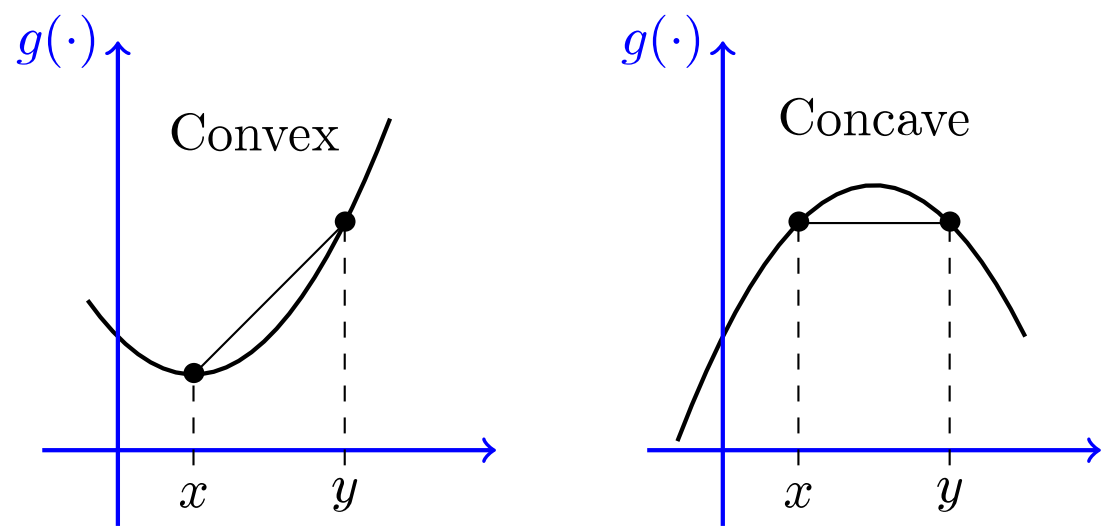
\includegraphics[scale=0.25]{images/convexvsconcave.png}
\end{figure}

\noindent
If the function is twice-differentiable, then it is convex if its second derivative is non-negative.
To find out if a multivariate function is convex or concave, we can use the following table:

\begin{figure}[h]
    \centering
    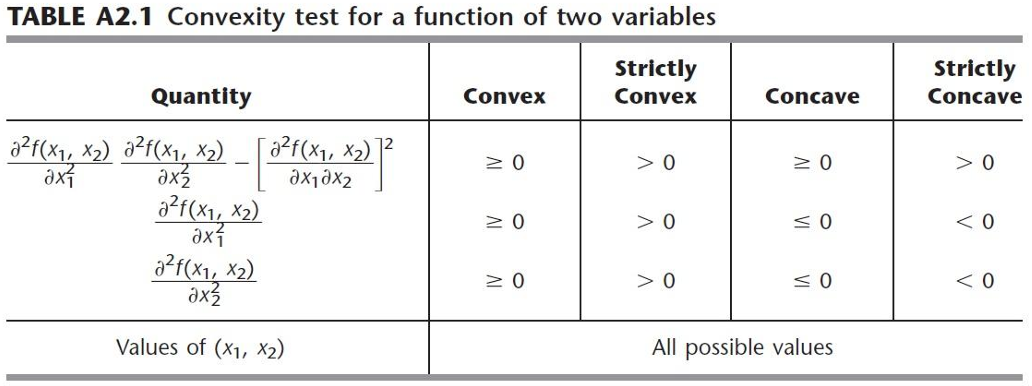
\includegraphics[scale=0.7]{images/convexitytable.PNG}
    \\(given on exam)
\end{figure}

\noindent
Some useful properties to remember are that the negation of a convex function is concave, and that the sum of two convex functions is convex.

\newpage
\subsubsection{Convex Sets}
A convex set is a set where the line segment between any two points in the set lies entirely within the set:

\begin{figure}[h]
    \centering
    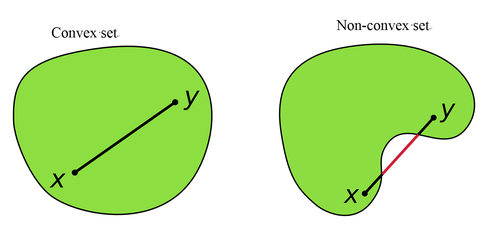
\includegraphics[scale=0.6]{images/convexitysets.png}
\end{figure}

\noindent
A critical property of convex sets is that the intersection of any number of convex sets is also convex.
This is why the feasible region of any linear program is convex, and, more importantly, why any nonlinear program with \textbf{convex constraints} will describe a convex feasible region.
A constraint is convex if it is of the form $g(x) \leq d$, where $g(x)$ is convex and $d$ is constant.

\noindent
\\
The reason we want convex or concave functions is that they have a single optimum.
The reason we want a convex feasible region is that this prevents "difficult to reach parts" in the feasible region, making the problem easier to solve.
Convex programming requires both of these properties.
This makes it far more tractable than non-convex programming.

\subsection{Unconstrained Optimization}
The simplest form of nonlinear programming is \textbf{unconstrained optimization}, where we only have an objective function to optimize.

\subsubsection{Single-Variable Optimization}
The find the optimum of a single-variable function, we can simply set the first derivative to zero and solve for $x$.
However, even for single-variable functions, this can be difficult to do analytically.
The more attractive option is to use numerical methods, which iteratively converge to the optimum.
One of these numerical methods is the \textbf{Bisection Method}, which can find the optimum of a function $f(x)$, given its derivative $f^\prime(x)$ and an interval $[a, b]$ where $f^\prime(a)$ and $f^\prime(b)$ have different signs:

\begin{enumerate}
    \item Calculate $c$, the midpoint of the interval.
    \item Calculate $f^\prime(c)$.
    \item If convergence is reached (i.e. $f^\prime(c)$ is sufficiently close to zero), return $c$.
    \item Else, examine the sign $f^\prime(c)$ and replace either $a$ or $b$ with $c$ such that there is still a zero crossing in the new interval. Repeat from step 1.
\end{enumerate}

\newpage
\subsubsection{Multi-Variable Optimization}
Just like with single-variable optimization, numerical methods are often used for multi-variable optimization.
One of the most common methods is the \textbf{Gradient Search} method.
The idea is to start at a point $x_0$ and move in the direction of the most positive gradient until it reaches a point where the gradient is zero.

\subsection{Constrained Optimization}
Constrained optimization is the more general form of nonlinear programming, where we have an objective function to optimize containing decision variables $<x_1, x_2, ... , x_n>$, subject to a set of constraints:
\begin{align*}
    &\mathrm{max} \quad Z = f(x) \\[2pt]
    &\mathrm{s.t.} \quad 
    \begin{array}[t]{r c l}
        g_i(x) & \leq & b_i \\
        x & \geq & 0
    \end{array}
\end{align*}

\subsubsection{KKT Conditions}
The \textbf{Karush-Kuhn-Tucker (KKT) conditions} are necessary conditions for a point to be an optimum of a nonlinear program.
In a convex program, the KKT conditions are also sufficient (i.e. if the KKT conditions are satisfied, then the point is an optimum).

\noindent
\\
Consider a \textit{maximization} nonlinear program with $n$ decision variables and $m$ functional constraints.
Assuming $f(x)$ and $g_i(x)$ are differentiable, then $x = (x_1^*, x_2^*, ... , x_n^*)$ is an optimum solution if there exist $m$ numbers $u_1, u_2, ... , u_m$ such that all the following KKT conditions are satisfied:

\begin{enumerate}
    \item \makebox[6cm][l]{$\displaystyle\frac{\partial f}{\partial x_j} - \displaystyle\sum\limits_{i = 1}^m u_i \displaystyle\frac{\partial g_i}{\partial x_j} \leq 0$} for $j = 1, 2, ... , n$
    \item \makebox[6cm][l]{$x_j^* \left( \displaystyle\frac{\partial f}{\partial x_j} - \displaystyle\sum\limits_{i = 1}^m u_i \displaystyle\frac{\partial g_i}{\partial x_j} \right) = 0$} for $j = 1, 2, ... , n$
    \item \makebox[6cm][l]{$g_i(x^*) - b_i \leq 0$} for $i = 1, 2, ... , m$
    \item \makebox[6cm][l]{$u_i[g_i(x^*) - b_i] = 0$} for $i = 1, 2, ... , m$
    \item \makebox[6cm][l]{$x_j^* \geq 0$} for $j = 1, 2, ... , n$
    \item \makebox[6cm][l]{$u_i \geq 0$} for $i = 1, 2, ... , m$
\end{enumerate}

\noindent
Note that these KKT conditions only apply to maximization problems.
If you have a minimization problem, you can simply multiply the objective function by $-1$ and apply the KKT conditions for maximization.

\newpage
\noindent
To illustrate the KKT conditions, consider the following example:
\begin{align*}
    &\mathrm{max} \quad f(x) = \ln(x_1 + 1) + x_2 \\[2pt]
    &\mathrm{s.t.} \quad 
    \begin{array}[t]{r c l}
        2x_1 + x_2 & \leq & 3 \\
        x_1, x_2 & \geq & 0
    \end{array}
\end{align*}

\noindent
Here $n = 2$ and $m = 1$.
$f(x)$ is concave and $g_1(x)$ is convex, so this is a convex program.
The KKT conditions for this problem are as follows:

\begin{itemize}[wide=10pt]
    \item[1($j = 1$).]{\makebox[5cm]{$\displaystyle\frac{1}{x_1 + 1} - 2u_1 \leq 0$}}
    \item[2($j = 1$).]{\makebox[5cm]{$x_1 \left( \displaystyle\frac{1}{x_1 + 1} - 2u_1 \right) = 0$}}
    \item[1($j = 2$).]{\makebox[5cm]{$1 - u_1 \leq 0$}}
    \item[2($j = 2$).]{\makebox[5cm]{$x_2 (1 - u_1) = 0$}}
    \item[3.]{\makebox[7.5cm]{$2x_1 + x_2 - 3 \leq 0$}}
    \item[4.]{\makebox[7.5cm]{$u_1(2x_1 + x_2 - 3) = 0$}}
    \item[5.]{\makebox[7.5cm]{$x_1 \geq 0, x_2 \geq 0$}}
    \item[6.]{\makebox[7.5cm]{$u_1 \geq 0$}}
\end{itemize}

\noindent
We can solve these KKT conditions to find the optimal solution to the problem as follows:

\begin{enumerate}
    \item $u_1 \geq 1$, from condition 1($j = 2$), $x_1 \geq 0$, from condition 5.
    \item Therefore, $\displaystyle\frac{1}{x_1 + 1} - 2u_1 < 0$.
    \item Therefore, $x_1 = 0$, from condition 2($j = 1$).
    \item $u_1 \neq 0$ implies $2x_1 + x_2 - 3 = 0$, from condition 4.
    \item Steps 3 and 4 imply $x_2 = 3$.
    \item $x_2 \neq 0$ implies $u_1 = 1$, from condition 2($j = 2$).
    \item No conditions are violated by $x_1 = 0, x_2 = 3, u_1 = 1$.
\end{enumerate}

\end{document}
